\documentclass[a4paper]{article}

\def\npart {IV}
\def\nterm {Easter}
\def\nyear {2017}
\def\nlecturer {M.\ Burger}
\def\ncourse {Bounded Cohomology}
\def\nnotready{}

% Imports
\ifx \nextra \undefined
  \usepackage[pdftex,
    hidelinks,
    pdfauthor={Dexter Chua},
    pdfsubject={Cambridge Maths Notes: Part \npart\ - \ncourse},
    pdftitle={Part \npart\ - \ncourse},
  pdfkeywords={Cambridge Mathematics Maths Math \npart\ \nterm\ \nyear\ \ncourse}]{hyperref}
  \title{Part \npart\ - \ncourse}
\else
  \usepackage[pdftex,
    hidelinks,
    pdfauthor={Dexter Chua},
    pdfsubject={Cambridge Maths Notes: Part \npart\ - \ncourse\ (\nextra)},
    pdftitle={Part \npart\ - \ncourse\ (\nextra)},
  pdfkeywords={Cambridge Mathematics Maths Math \npart\ \nterm\ \nyear\ \ncourse\ \nextra}]{hyperref}

  \title{Part \npart\ - \ncourse \\ {\Large \nextra}}
\fi

\author{Lectured by \nlecturer \\\small Notes taken by Dexter Chua}
\date{\nterm\ \nyear}

\usepackage{alltt}
\usepackage{amsfonts}
\usepackage{amsmath}
\usepackage{amssymb}
\usepackage{amsthm}
\usepackage{booktabs}
\usepackage{caption}
\usepackage{enumitem}
\usepackage{fancyhdr}
\usepackage{graphicx}
\usepackage{mathtools}
\usepackage{microtype}
\usepackage{multirow}
\usepackage{pdflscape}
\usepackage{pgfplots}
\usepackage{siunitx}
\usepackage{tabularx}
\usepackage{tikz}
\usepackage{tkz-euclide}
\usepackage[normalem]{ulem}
\usepackage[all]{xy}

\pgfplotsset{compat=1.12}

\pagestyle{fancyplain}
\lhead{\emph{\nouppercase{\leftmark}}}
\ifx \nextra \undefined
  \rhead{
    \ifnum\thepage=1
    \else
      \npart\ \ncourse
    \fi}
\else
  \rhead{
    \ifnum\thepage=1
    \else
      \npart\ \ncourse\ (\nextra)
    \fi}
\fi
\usetikzlibrary{arrows}
\usetikzlibrary{decorations.markings}
\usetikzlibrary{decorations.pathmorphing}
\usetikzlibrary{positioning}
\usetikzlibrary{fadings}
\usetikzlibrary{intersections}
\usetikzlibrary{cd}

\newcommand*{\Cdot}{\raisebox{-0.25ex}{\scalebox{1.5}{$\cdot$}}}
\newcommand {\pd}[2][ ]{
  \ifx #1 { }
    \frac{\partial}{\partial #2}
  \else
    \frac{\partial^{#1}}{\partial #2^{#1}}
  \fi
}

% Theorems
\theoremstyle{definition}
\newtheorem*{aim}{Aim}
\newtheorem*{axiom}{Axiom}
\newtheorem*{claim}{Claim}
\newtheorem*{cor}{Corollary}
\newtheorem*{defi}{Definition}
\newtheorem*{eg}{Example}
\newtheorem*{fact}{Fact}
\newtheorem*{law}{Law}
\newtheorem*{lemma}{Lemma}
\newtheorem*{notation}{Notation}
\newtheorem*{prop}{Proposition}
\newtheorem*{thm}{Theorem}

\renewcommand{\labelitemi}{--}
\renewcommand{\labelitemii}{$\circ$}
\renewcommand{\labelenumi}{(\roman{*})}

\let\stdsection\section
\renewcommand\section{\newpage\stdsection}

% Strike through
\def\st{\bgroup \ULdepth=-.55ex \ULset}

% Maths symbols
\newcommand{\bra}{\langle}
\newcommand{\ket}{\rangle}

\newcommand{\N}{\mathbb{N}}
\newcommand{\Z}{\mathbb{Z}}
\newcommand{\Q}{\mathbb{Q}}
\renewcommand{\H}{\mathbb{H}}
\newcommand{\R}{\mathbb{R}}
\newcommand{\C}{\mathbb{C}}
\newcommand{\Prob}{\mathbb{P}}
\renewcommand{\P}{\mathbb{P}}
\newcommand{\E}{\mathbb{E}}
\newcommand{\F}{\mathbb{F}}
\newcommand{\cU}{\mathcal{U}}
\newcommand{\RP}{\mathbb{RP}}
\newcommand{\CP}{\mathbb{CP}}

\newcommand{\ph}{\,\cdot\,}

\DeclareMathOperator{\sech}{sech}
\DeclareMathOperator{\cosech}{cosech}
\DeclareMathOperator{\cosec}{cosec}

\DeclareMathOperator{\covol}{covol}
\DeclareMathOperator{\vol}{vol}

\let\Im\relax
\let\Re\relax
\DeclareMathOperator{\Im}{Im}
\DeclareMathOperator{\Re}{Re}
\DeclareMathOperator{\im}{im}
\DeclareMathOperator{\image}{image}
\DeclareMathOperator{\Ann}{Ann}

\DeclareMathOperator*{\res}{res}
\DeclareMathOperator{\Res}{Res}
\DeclareMathOperator{\Ind}{Ind}

\DeclareMathOperator{\tr}{tr}
\DeclareMathOperator{\diag}{diag}
\DeclareMathOperator{\rank}{rank}
\DeclareMathOperator{\card}{card}
\DeclareMathOperator{\spn}{span}
\DeclareMathOperator{\adj}{adj}

\DeclareMathOperator{\erf}{erf}
\DeclareMathOperator{\erfc}{erfc}

\DeclareMathOperator{\ord}{ord}
\DeclareMathOperator{\Sym}{Sym}

\DeclareMathOperator{\sgn}{sgn}
\DeclareMathOperator{\orb}{orb}
\DeclareMathOperator{\stab}{stab}
\DeclareMathOperator{\ccl}{ccl}

\DeclareMathOperator{\lcm}{lcm}
\DeclareMathOperator{\hcf}{hcf}

\DeclareMathOperator{\Int}{Int}
\DeclareMathOperator{\id}{id}

\DeclareMathOperator{\betaD}{beta}
\DeclareMathOperator{\gammaD}{gamma}
\DeclareMathOperator{\Poisson}{Poisson}
\DeclareMathOperator{\binomial}{binomial}
\DeclareMathOperator{\multinomial}{multinomial}
\DeclareMathOperator{\Bernoulli}{Bernoulli}
\DeclareMathOperator{\like}{like}

\DeclareMathOperator{\var}{var}
\DeclareMathOperator{\cov}{cov}
\DeclareMathOperator{\bias}{bias}
\DeclareMathOperator{\mse}{mse}
\DeclareMathOperator{\corr}{corr}

\DeclareMathOperator{\otp}{otp}
\DeclareMathOperator{\dom}{dom}

\DeclareMathOperator{\Root}{Root}
\DeclareMathOperator{\supp}{supp}
\DeclareMathOperator{\rel}{rel}
\DeclareMathOperator{\Hom}{Hom}
\DeclareMathOperator{\Aut}{Aut}
\DeclareMathOperator{\Gal}{Gal}
\DeclareMathOperator{\Mat}{Mat}
\DeclareMathOperator{\End}{End}
\DeclareMathOperator{\Char}{char}
\DeclareMathOperator{\ev}{ev}
\DeclareMathOperator{\St}{St}
\DeclareMathOperator{\Lk}{Lk}
\DeclareMathOperator{\disc}{disc}
\DeclareMathOperator{\Isom}{Isom}
\DeclareMathOperator{\length}{length}
\DeclareMathOperator{\energy}{energy}
\DeclareMathOperator{\area}{area}
\DeclareMathOperator{\Syl}{Syl}
\DeclareMathOperator{\cl}{cl}
\DeclareMathOperator{\fix}{fix}

\newcommand{\GL}{\mathrm{GL}}
\newcommand{\SL}{\mathrm{SL}}
\newcommand{\PGL}{\mathrm{PGL}}
\newcommand{\PSL}{\mathrm{PSL}}
\newcommand{\PSU}{\mathrm{PSU}}
\newcommand{\Or}{\mathrm{O}}
\newcommand{\SO}{\mathrm{SO}}
\newcommand{\U}{\mathrm{U}}
\newcommand{\SU}{\mathrm{SU}}

\renewcommand{\d}{\mathrm{d}}
\newcommand{\D}{\mathrm{D}}

\tikzset{->/.style = {decoration={markings,
                                  mark=at position 1 with {\arrow[scale=2]{latex'}}},
                      postaction={decorate}}}
\tikzset{<-/.style = {decoration={markings,
                                  mark=at position 0 with {\arrowreversed[scale=2]{latex'}}},
                      postaction={decorate}}}
\tikzset{<->/.style = {decoration={markings,
                                   mark=at position 0 with {\arrowreversed[scale=2]{latex'}},
                                   mark=at position 1 with {\arrow[scale=2]{latex'}}},
                       postaction={decorate}}}
\tikzset{->-/.style = {decoration={markings,
                                   mark=at position #1 with {\arrow[scale=2]{latex'}}},
                       postaction={decorate}}}
\tikzset{-<-/.style = {decoration={markings,
                                   mark=at position #1 with {\arrowreversed[scale=2]{latex'}}},
                       postaction={decorate}}}

\tikzset{circ/.style = {fill, circle, inner sep = 0, minimum size = 3}}
\tikzset{mstate/.style={circle, draw, blue, text=black, minimum width=0.7cm}}

\definecolor{mblue}{rgb}{0.2, 0.3, 0.8}
\definecolor{morange}{rgb}{1, 0.5, 0}
\definecolor{mgreen}{rgb}{0.1, 0.4, 0.2}
\definecolor{mred}{rgb}{0.5, 0, 0}

\def\drawcirculararc(#1,#2)(#3,#4)(#5,#6){%
    \pgfmathsetmacro\cA{(#1*#1+#2*#2-#3*#3-#4*#4)/2}%
    \pgfmathsetmacro\cB{(#1*#1+#2*#2-#5*#5-#6*#6)/2}%
    \pgfmathsetmacro\cy{(\cB*(#1-#3)-\cA*(#1-#5))/%
                        ((#2-#6)*(#1-#3)-(#2-#4)*(#1-#5))}%
    \pgfmathsetmacro\cx{(\cA-\cy*(#2-#4))/(#1-#3)}%
    \pgfmathsetmacro\cr{sqrt((#1-\cx)*(#1-\cx)+(#2-\cy)*(#2-\cy))}%
    \pgfmathsetmacro\cA{atan2(#2-\cy,#1-\cx)}%
    \pgfmathsetmacro\cB{atan2(#6-\cy,#5-\cx)}%
    \pgfmathparse{\cB<\cA}%
    \ifnum\pgfmathresult=1
        \pgfmathsetmacro\cB{\cB+360}%
    \fi
    \draw (#1,#2) arc (\cA:\cB:\cr);%
}
\newcommand\getCoord[3]{\newdimen{#1}\newdimen{#2}\pgfextractx{#1}{\pgfpointanchor{#3}{center}}\pgfextracty{#2}{\pgfpointanchor{#3}{center}}}

\def\Xint#1{\mathchoice
   {\XXint\displaystyle\textstyle{#1}}%
   {\XXint\textstyle\scriptstyle{#1}}%
   {\XXint\scriptstyle\scriptscriptstyle{#1}}%
   {\XXint\scriptscriptstyle\scriptscriptstyle{#1}}%
   \!\int}
\def\XXint#1#2#3{{\setbox0=\hbox{$#1{#2#3}{\int}$}
     \vcenter{\hbox{$#2#3$}}\kern-.5\wd0}}
\def\ddashint{\Xint=}
\def\dashint{\Xint-}


\newcommand\QH{\mathcal{QH}}
\newcommand\scl{\mathrm{scl}}
\newcommand\Homeo{\mathrm{Homeo}}
\newcommand\Rot{\mathrm{Rot}}
\newcommand\Free{F}

\begin{document}
\maketitle
{\small
\setlength{\parindent}{0em}
\setlength{\parskip}{1em}

The cohomology of a group or a topological space in degree $k$ is a real vector space which describes the ``holes'' bounded by k dimensional cycles and encodes their relations. Bounded cohomology is a refinement which provides these vector spaces with a (semi) norm and hence topological objects acquire mysterious numerical invariants. This theory, introduced in the beginning of the 80's by M.\ Gromov, has deep connections with the geometry of hyperbolic groups and negatively curved manifolds. For instance, hyperbolic groups can be completely characterized by the ``size'' of their bounded cohomology.

The aim of this course is to give an introduction to the bounded cohomology of groups, and treat more in detail one of its important applications to the study of groups acting by homeomorphisms on the circle. More precisely we will treat the following topics:
\begin{enumerate}
  \item Ordinary and bounded cohomology of groups: meaning of these objects in low degrees, that is, zero, one and two; relations with quasimorphisms. Proof that the bounded cohomology in degree two of a non abelian free group contains an isometric copy of the Banach space of bounded sequences of reals. Examples and meaning of bounded cohomology classes of geometric origin with non trivial coefficients.

  \item Actions on the circle, the bounded Euler class: for a group acting by orientation preserving homeomorphisms of the circle, Ghys has introduced an invariant, the bounded Euler class of the action, and shown that it characterizes (minimal) actions up to conjugation. We will treat in some detail this work as it leads to important applications of bounded cohomology to the question of which groups can act non trivially on the circle: for instance $\SL(2,\Z)$ can, while lattices in ``higher rank Lie groups'', like $\SL(n,\Z)$ for $n$ at least $3$, can't.

  \item Amenability and resolutions: we will set up the abstract machinery of resolutions and the notions of injective modules in ordinary as well as bounded cohomology; this will provide a powerful way to compute these objects in important cases. A fundamental role in this theory is played by various notions of amenability; the classical notion of amenability for a group, and amenability of a group action on a measure space, due to R.\ Zimmer. The goal is then to describe applications of this machinery to various rigidity questions, and in particular to the theorem due, independently to Ghys, and Burger--Monod, that lattices in higher rank groups don't act on the circle.
\end{enumerate}

\subsubsection*{Pre-requisites}
Prerequisites for this course are minimal: no prior knowledge of group cohomology of any form is needed; we'll develop everything we need from scratch. It is however an advantage to have a ``zoo'' of examples of infinite groups at one's disposal: for example free groups and surface groups. In the third part, we'll need basic measure theory; amenability and ergodic actions will play a role, but there again everything will be built up on elementary measure theory.

The basic reference for this course is R.\ Frigerio, ``Bounded cohomology of discrete groups'', \href{https://arxiv.org/abs/1611.08339}{arXiv:1611.08339}, and for part 3, M.\ Burger \& A.\ Iozzi, ``A useful formula from bounded cohomology'', available at: \url{https://people.math.ethz.ch/~iozzi/publications.html}.%
}
\tableofcontents

\section{Quasi-homomorphisms}
\subsection{Quasi-homomorphisms}
In this chapter, $A$ will denote $\Z$ or $\R$. Let $G$ be a group. The usual definition of a group homomorphism $f: G \to A$ requires that for all $x, y \in G$, we have
\[
  f(xy) = f(x) + f(y).
\]
In a quasi-homomorphism, we replace the equality with a weaker notion, and allow for some ``errors''.

\begin{defi}[Quasi-homomorphism]\index{quasi-homomorphism}
  Let $G$ be a group. A function $f: G \to A$ is a \emph{quasi-homomorphism} if the function
  \begin{align*}
    \d f: G \times G &\to A\\
    (x, y) &\mapsto f(x) + f(y) - f(xy)
  \end{align*}
  is \emph{bounded}. We define the \term{defect}\index{quasi-homomorphism!defect} of $f$ to be
  \[
    D(f) = \sup_{x, y \in G} |\d f(x, y)|.
  \]
  We write \term{$\QH(G, A)$} for the $A$-module of quasi-homomorphisms.
\end{defi}

\begin{eg}
  Every homomorphism is a quasi-homomorphism with $D(f) = 0$. Conversely, a quasi-homomorphism with $D(f) = 0$ is a homomorphism.
\end{eg}

We can obtain some ``trivial'' quasi-homomorphisms as follows --- we take any homomorphism, and then edit finitely many values of the homomorphism. Then this is a quasi-homomorphism. More generally, we can add any bounded function to a quasi-homomorphism and still get a quasi-homomorphism.

\begin{notation}
  We write\index{$\ell^\infty(G, A)$}
  \[
    \ell^\infty(G, A) = \{f: G \to A: \text{$f$ is bounded}\}.
  \]
\end{notation}

Thus, we are largely interested in the quasi-homomorphisms modulo $\ell^\infty(G, A)$. Often, we also want to quotient out by the genuine homomorphisms, and obtain
\[
  \frac{\QH(G, A)}{\ell^\infty(G, A) + \Hom(G, A)}.
\]
This contains subtle algebraic and geometric information about $G$, and we will later see this is related to the second bounded cohomology $H_b^2(G, A)$.

We first prove a few elementary facts about quasi-homomorphisms. The first task is to find canonical representatives of the classes in the quotient $\QH(G, \R)/\ell^\infty (G, \R)$.

\begin{defi}[Homogeneous function]\index{homegeneous function}\index{function!homogeneous}
  A function $f: G \to \R$ is \emph{homogeneous} if for all $n \in \Z$ and $g \in G$, we have $f(g^n) = n f(g)$.
\end{defi}

\begin{lemma}
  Let $f \in \QH(G, A)$. Then for every $g \in G$, the limit
  \[
    Hf(g) = \lim_{n \to \infty} \frac{f(g^n)}{n}
  \]
  exists in $\R$. Moreover,
  \begin{enumerate}
    \item $Hf: G \to \R$ is a homogeneous quasi-homomorphism.
    \item $f - Hf \in \ell^\infty(G, \R)$.
  \end{enumerate}
\end{lemma}
% So this $Hf$ gives us a ``preferred'' representative for each class in$\QH(G, \R) / \ell^\infty(G, \R)$.

\begin{proof}
  We iterate the quasi-homomorphism property
  \[
    |f(ab) - f(a) - f(b)| \leq D(f).
  \]
  Then, viewing $g^{mn} = g^m \cdots g^m$, we obtain
  \[
    |f(g^{mn}) - n f(g^m)| \leq (n - 1) D(f).
  \]
  Similarly, we also have
  \[
    |f(g^{mn}) -m f(g^n)| \leq (m - 1) D(f).
  \]
  Thus, dividing by $nm$, we find
  \begin{align*}
    \left|\frac{f(g^{mn})}{nm} - \frac{f(g^m)}{m}\right| &\leq \frac{1}{m} D(f)\\
    \left|\frac{f(g^{mn})}{nm} - \frac{f(g^n)}{n}\right| &\leq \frac{1}{n} D(f).
  \end{align*}
  So we find that
  \[
    \left|\frac{f(g^n)}{n} - \frac{f(g^m)}{m}\right| \leq \left(\frac{1}{m} + \frac{1}{n} \right) D(f).\tag{$*$}
  \]
  Hence the sequence $\frac{f(g^n)}{n}$ is Cauchy, and the limit exists.

  The fact that $Hf$ is a quasi-homomorphism follows from the second assertion. To prove the second assertion, we can just take $n = 1$ in $(*)$ and take $m \to \infty$. Then we find
  \[
    |f(g) - Hf(g)| \leq D(f).
  \]
  So this shows that $f - Hf$ is bounded, hence $Hf$ is a quasi-homomorphism.

  The homogeneity is left as an easy exercise.
\end{proof}

\begin{notation}
  We write \term{$\QH_h(G, \R)$} for the vector space of homogeneous quasi-homomorphisms $G \to \R$.
\end{notation}

Then the above theorem gives
\begin{cor}
  We have
  \[
    \QH(G, \R) = \QH_h(G, \R) \oplus \ell^\infty(G, \R)
  \]
\end{cor}

\begin{proof}
  Indeed, observe that a bounded homogeneous quasi-homomorphism must be identically zero.
\end{proof}

Thus, if we want to study $\QH(G, \R)$, it suffices to just look at the homogeneous quasi-homomorphisms. It turns out these have some very nice perhaps-unexpected properties.
\begin{lemma}
  Let $f: G \to \R$ be a homogeneous quasi-homomorphism.
  \begin{enumerate}
    \item We have $f(xyx^{-1}) = f(y)$ for all $x, y \in G$.
    \item If $G$ is abelian, then $f$ is in fact a homomorphism. Thus
      \[
        \QH_h(G, \R) = \Hom(G, \R).
      \]
  \end{enumerate}
\end{lemma}
Thus, quasi-homomorphisms are only interesting for non-abelian groups.

\begin{proof}\leavevmode
  \begin{enumerate}
    \item Note that for any $x$, the function
      \[
        y \mapsto f(xyx^{-1})
      \]
      is a homogeneous quasi-homomorphism. By the previous corollary, it suffices to show that the function
      \[
        y \mapsto f(xyx^{-1}) - f(y)
      \]
      is a bounded homogeneous quasi-homomorphism, hence zero. This is just an iteration of the quasi-homomorphism property. We have
      \[
        |f(xyx^{-1}) - f(y)| \leq |f(x) + f(y) + f(x^{-1}) - f(y)| + 2D(f) = 2D(f),
      \]
      using the fact that $f(x^{-1}) = -f(x)$ by homogeneity.
    \item If $x$ and $y$ commute, then $(xy)^n = x^n y^n$. So we can use homogeneity to write
      \begin{align*}
        |f(xy) - f(x) - f(y)| &= \frac{1}{n} |f((xy)^n) - f(x^n) - f(y^n)|\\
        &= \frac{1}{n} | f(x^n y^n) - f(x^n) - f(y^n)|\\
        &\leq \frac{1}{n} D(f).
      \end{align*}
      Since $n$ is arbitrary, the difference must vanish.
  \end{enumerate}
\end{proof}

The case of $\QH(G, \Z)/\ell^\infty(G, \Z)$ is more complicated. For example, we have the following nice result:
\begin{eg}
  Given $\alpha \in \R$, define the map $g_\alpha: \Z \to \Z$ by
  \[
    g_\alpha(m) = [m\alpha].
  \]
  Then this is a homomorphism, and the map
  \begin{align*}
    \R &\longrightarrow \frac{\QH(\Z, \Z)}{\ell^\infty(\Z, \Z)}\\
    \alpha &\longmapsto g_\alpha
  \end{align*}
  is an isomorphism. This gives a further isomorphism
  \[
    \R \cong \frac{\QH(\Z, \Z)}{\ell^\infty(\Z, \Z) + \Hom(\Z, \Z)}.
  \]
\end{eg}

We next turn to the case $G = \Free_2$, the free group on two generators $a, b$. We will try to work out explicitly a lot of non-trivial elements of $\QH(\Free_2, \R)$. In general, when we try to construct quasi-homomorphisms, what we manage to get are \emph{not} homogeneous. So when we construct several quasi-homomorphisms, it takes some non-trivial work to show that they are distinct. Our construction will be one such that this is relatively easy to see.

Consider the vector space:
\[
  \ell_{\mathrm{odd}}^\infty (\Z) = \{\alpha: \Z \to \R : \alpha \text{ bounded and } \alpha(-n) = -\alpha (n)\}.
\]
Note that in particular, we have $\alpha(0) = 0$.

Given $\alpha, \beta \in \ell_{\mathrm{odd}}^\infty(\Z)$, we define a quasi-homomorphisms $f_{\alpha, \beta} : \Free_2 \to \R$ as follows --- given a reduced word $w = a^{n_1} b^{m_1} \cdots a^{n_k}b^{m_k}$, we let
\[
  f_{\alpha, \beta}(w) = \sum_{i= 1}^k \alpha(n_i) + \sum_{j = 1}^k \beta(m_j).
\]
Allowing for $n_1 = 0$ or $m_k = 0$, this gives a well-defined function $f_{\alpha,\beta}$ defined on all of $\Free_2$.

Let's see what this does on some special sequences.
\begin{eg}
  We have
  \[
    f_{\alpha, \beta}(a^n) = \alpha(n),\quad f_{\alpha, \beta}(b^m) = \beta(m),
  \]
  and these are bounded functions of $n, m$.
\end{eg}
So we see that $f_{\alpha, \beta}$ is never homogeneous unless $\alpha = \beta = 0$.

\begin{eg}
  Pick $k_1, k_2, n \not= 0$, and set
  \[
    w = a^{nk_1} b^{nk_2} (b^{k_2}a^{k_1})^{-n} = a^{nk_1} b^{nk_2} \underbrace{a^{-k_1} b^{-k_2} \cdots a^{-k_1} b^{-k_2}}_{n\text{ times}}.
  \]
  This is now in reduced form. So we have
  \[
    f_{\alpha, \beta}(w) = \alpha(n k_1) + \beta (n k_2) - n \alpha(k_1) - n \beta(k_2).
  \]
\end{eg}
This example is important. If $\alpha(k_1) + \beta(k_2) \not= 0$, then this is an unbounded function as $n \to \infty$. However, we know any genuine homomoprhisms $f: \Free_2 \to \R$ must factor through the abelianization, and $w$ vanishes in the abelianization. So this suggests our $f_{\alpha, \beta}$ is in some sense very far away from being a homomorphism.

\begin{thm}[P.\ Rolli, 2009]
  The function $f_{\alpha, \beta}$ is a quasi-homomorphism, and the map
  \[
    \ell^\infty_{\mathrm{odd}} (\Z) \oplus \ell^\infty_{\mathrm{odd}}(\Z) \to \frac{\QH(\Free_2, \R)}{\ell^\infty(\Free_2, \R) + \Hom(\Free_2, \R)}
  \]
  is injective.
\end{thm}
This tells us there are a lot of non-trivial elements in $\QH(\Free_2, \R)$.

The advantage of this construction is that the map above is a \emph{linear} map. So to see it is injective, it suffices to see that it has trivial kernel.
\begin{proof}
  Let $\alpha, \beta \in \ell_{\mathrm{odd}}^\infty (\Z, \R)$, and define $f_{\alpha, \beta}$ as before. By staring at it long enough, we find that
  \[
    |f(xy) - f(x) - f(y)| \leq 3 \max (\|\alpha\|_\infty, \|\beta\|_\infty),
  \]
  and so it is a quasi-homomorphism. The main idea is that
  \[
    f(b^n) + f(b^{-n}) = f(a^n) + f(a^{-n}) = 0
  \]
  by oddness of $\alpha$ and $\beta$. So when we do the word reduction in the product, the amount of error we can introduce is at most $3 \max (\|\alpha\|_\infty, \|\beta\|_\infty)$.

  To show that the map is injective, suppose
  \[
    f_{\alpha, \beta} = \varphi + h,
  \]
  where $\varphi: \Free_2 \to \R$ is bounded and $h: \Free_2 \to \R$ is a homomorphism. Then we must have
  \[
    h(a^\ell) = f(a^\ell) - \varphi(a^\ell) = \alpha(\ell) - \psi(a^\ell),
  \]
  which is bounded. So the map $\ell \mapsto h(a^\ell) = \ell h(a)$ is bounded, and so $h(a) = 0$. Similarly, $h(b) = 0$. So $h \equiv 0$. In other words, $f_{\alpha, \beta}$ is bounded.

  Finally,
  \[
    f((a^{\ell_1} b^{\ell_2})^k) = k (\alpha(\ell_1) + \beta(\ell_2)) = 0.
  \]
  Since this is bounded, we must have $\alpha(\ell_1) + \beta(\ell_2) = 0$ for all $\ell_1, \ell_2 \not= 0$. Using the fact that $\alpha$ and $\beta$ are odd, this easily implies that $\alpha(\ell_1) = \beta(\ell_2) = 0$ for all $1$ and $2$.

% We say $x \in \F_2$ is a power if $x = a^k$ or $b^k$ for some $k \in \Z \setminus \{0\}$.
%
% Every $x \in \F_2$ has a unique shortest factorization into powers. If $x = x_1 \cdots x_n$ is the shortest factorization into powers, then
% \[
% f(x) = \sum_{i = 1}^n f(x_i).
% \]
% Let $x, y \in \F_2$ with shortest factorzation
% \begin{align*}
% x &= x_0 \cdots x_n\\
% y &= y_0 \cdots y_m
% \end{align*}
% Then we have
% \[
% xy = x_1 \cdots x_n y_1 \cdots y_n.
% \]
% Now if $x_n y_0 = e$, then $f(x_n) + f(y_0) = 0$ by oddness. Suppose that
% \[
% x_n y_0 = x_{n - 1} y_1 = .. = x_{n - (r - 2)} y_{r - 2} = e,
% \]
% and
% \[
% x_{n - (r - 1)} y_{r - 1} = \zeta,
% \]
% and
% \[
% xy = x_0 \cdots x_{n - r} \zeta y_r \cdots y_m
% \]
% is a factorization into powers. Then we have
% \[
% f(y) = \sum_{i = 0}^n f(x_i) = \sum_{i = 0}^{n - r} f(x_i) + f(x_{n - (r - 1)}) + \sum_{j = 0}^r f(x_{n - j})
% \]
\end{proof}

More generally, we have the following theorem, which we shall not prove:
\begin{thm}[Hull--Osin 2013]
  The space
  \[
    \frac{\QH(G, \R)}{\ell^\infty(G, \R) + \Hom(G, \R)}
  \]
  is infinite-dimensional if $G$ is acylindrically hyperbolic.
\end{thm}

\subsection{Relation to commutators}
A lot of interesting information about quasi-homomorphisms can be captured by considering commutators. Recall that we write
\[
  [x, y] = xyx^{-1}y^{-1}.
\]
If $f$ is a genuine homomorphisms, then it vanishes on all commutators, since the codomain is abelian. For \emph{homogeneous} quasi-homomorphisms, we can bound the value of $f$ by the defect:
\begin{lemma}
  If $f$ is a homogeneous quasi-homomorphism and $x, y \in G$, then
  \[
    |f([x, y])| \leq D(f).
  \]
\end{lemma}
For non-homogeneous ones, the value of $f$ on a commutator is still bounded, but requires a bigger bound.

\begin{proof}
  By definition of $D(f)$, we have
  \[
    |f([x, y]) - f(xyx^{-1}) - f(y^{-1})| \leq D(f).
  \]
  But since $f$ is homogeneous, we have $f(xyx^{-1}) = f(y) = - f(y^{-1})$. So we are done.
\end{proof}

This bound is in fact the best we can obtain:
\begin{lemma}[Bavard, 1992]
  If $f$ is a homogeneous quasi-homomorphism, then
  \[
    \sup_{x, y} |f([x, y])| = D(f).
  \]
\end{lemma}
We will neither prove this nor use this --- it is merely for amusement.

For a general element $a \in [G, G]$, it need not be of the form $[x, y]$. We can define
\begin{defi}[Commutator length]\index{commutator length}
  Let $a \in [G, G]$. Then \emph{commutator length} \term{$\cl(a)$} is the word length with respect to the generators
  \[
    \{[x, y] : x, y \in G\}.
  \]
  In other words, it is the smallest $n$ such that
  \[
    a = [x_1, y_1][x_2, y_2] \cdots [x_n, y_n]
  \]
  for some $x_i, y_i \in G$.
\end{defi}

It is an easy inductive proof to show that
\begin{lemma}
  For $a \in [G, G]$, we have
  \[
    |f(a)| \leq 2D(f) \cl(a).
  \]
\end{lemma}

By homogeneity, it follows that
\[
  |f(a)| = \frac{1}{n} |f(a^n)| \leq 2 D(f) \frac{\cl(a^n)}{n}.
\]

\begin{defi}[Stable commutator length]\index{stable commutator length}
  The \emph{stable commutator length} is defined by
  \[
    \scl(a) = \lim_{n \to \infty} \frac{\cl(a^n)}{n}.
  \]
\end{defi}

Then we have
\begin{prop}
  \[
    |f(a)| \leq 2 D(f) \scl(a).
  \]
\end{prop}

\begin{eg}
  Consider $\Free_2$ with generators $a, b$. Then clearly we have
  \[
    \cl([a, b]) = 1.
  \]
  It is not hard to verify that we also have
  \[
    \cl([a, b]^2) = 2.
  \]
  But interestingly, this ``pattern'' doesn't extend to higher powers. By writing it out explicitly, we find that
  \[
    [x, y]^3 = [xyx^{-1}, y^{-1} xyx^{-2}] [y^{-1}xy, y^2].
  \]
\end{eg}
In general, something completely mysterious can happen as we raise the power, especially in more complicated groups.

Similar to the previous result by Bavard, the bound of $|f(a)|$ by $\scl(a)$ is sharp.
\begin{thm}[Bavard, 1992]
  For all $a \in [G, G]$, we have
  \[
    \scl(a) = \frac{1}{2} \sup_{\phi \in \QH_h(G, \R)} \frac{|\phi(a)|}{|D(\phi)|},
  \]
  where, of course, we skip over those $\phi \in \Hom(G, \R)$ in the supremum.
\end{thm}
We've seen some ``duality'' result of this sort before. Recall that if we have a Banach space $X$, then for $x \in X$, we have
\[
  \|x\|_X = \sup_{\phi \in X^*} \frac{|\phi(x)|}{\|\phi\|_{X^*}}.
\]
That wasn't a very exciting result --- one direction is by definition of $\|\phi\|_{X^*}$ and the other follows from Hahn--Banach. It is possible to view Bavard's theorem as a version of this duality, but that involves some complicated twisting.

\begin{eg}
  We have
  \[
    \scl([a, b]) = \frac{1}{2}.
  \]
  However, showing this is not very straightforward.
\end{eg}

\begin{cor}
  The stable commutator length vanishes identically iff every homogeneous quasi-homomorphism is a homomoprhism.
\end{cor}

Note that if $\cl$ is bounded, then we have $\scl \equiv 0$. There exists interesting groups with bounded $\cl$, such as nilpotent finitely-generated groups, and so these have $\QH_h(G, \R) = \Hom(G, \R)$. We might think that the groups with $\cl$ bounded are ``almost abelian'', but it turns out not.

\begin{thm}[Carder--Keller 1983]
  For $n \geq 3$, we have
  \[
    \SL(n, \Z) = [\SL(n, \Z), \SL(n, \Z)],
  \]
  and the commutator length is bounded.
\end{thm}

More generally, we have
\begin{thm}[D.\ Witte Morris, 2007]
  Let $\mathcal{O}$ be the ring of integers of some number field. Then $\cl: [\SL(n, \mathcal{O}), \SL(n, \mathcal{O})] \to \R$ is bounded iff $n \geq 3$ or $n = 2$ and $\mathcal{O}^\times$ is infinite.
\end{thm}
The groups $\SL(n, \mathcal{O})$ have a common property --- they are lattices in real semisimple Lie groups. In fact, we have

\begin{thm}[Burger--Monod, 2002]
  Let $\Gamma < G$ be an irreducible lattice in a connected semisimple group $G$ with finite center and rank $G \geq 2$. Then every homogeneous quasimorphism $\Gamma \to \R$ is $\equiv 0$.
\end{thm}

\begin{eg}
  If $\Gamma < \SL(n, \R)$ is a discrete subgroup such that $\Gamma \backslash \SL(n, \R)$ is compact, then it falls into the above class, and the rank condition is $n \geq 3$.
\end{eg}
It is in fact conjectured that
\begin{itemize}
  \item The commutator length is bounded.
  \item $\Gamma$ is boundedly generated, i.e.\ we can find generators $\{s_1, \cdots, s_k\}$ such that
    \[
      \Gamma = \bra s_1 \ket \bra s_2\ket \cdots \bra s_k\ket.
    \]
\end{itemize}

There is another theorem that seems completely unrelated to this, but actually uses the same technology.
\begin{thm}[Burger--Monod, 2009]
  Let $\Gamma$ be a finitely-generated group and let $\mu$ be a symmetric probability measure on $\Gamma$ whose support generates $\Gamma$. Then every class in $\QH(\Gamma, \R)/\ell^\infty(\Gamma, \R)$ has a unique $\mu$-harmonic representative. In addition, this harmonic representative $f$ satisfies the following:
  \[
    \|\d f\|_\infty \leq \|\d g\|_\infty
  \]
  for any $g \in f+ \ell^\infty(\Gamma, R)$.
\end{thm}
This is somewhat like the Hodge decomposition theorem.

\subsection{Poincare translation quasimorphism}
We will later spend quite a lot of time studying actions on the circle. Thus, we are naturally interested in the homeomorphism group of the sphere. We are mostly interested in orientation-preserving actions only. Thus, we need to define what it means for a homeomorphism $\varphi: S^1 \to S^1$ to be orientation-preserving.

The topologist will tell us that $\varphi$ induces a map
\[
  \varphi_*: H_1(S^1, \Z) \to H_1(S^1, \Z).
\]
Since the homology group is generated by the fundamental class $[S^1]$, invertibility of $\varphi_*$ implies $\varphi_*([S^1]) = \pm [S^1]$. Then we say $\varphi$ is orientation-preserving if $\varphi_*([S^1]) = [S^1]$.

However, this definition is practically useless if we want to do anything with it. Note that there is a natural covering map $\pi: \R \to S^1$ given by quotienting by $\Z$.

\begin{defi}[Positively-oriented triple]\index{positively-oriented triple}
  We say a triple of points $x_1, x_2, x_3 \in S^1$ is positively-oriented if they are distinct and ordered as follows:
  \begin{center}
    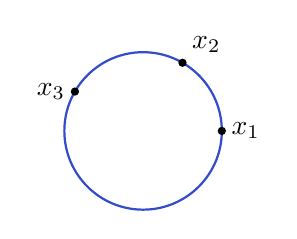
\begin{tikzpicture}
      \draw [mblue, thick] circle [radius=1];
      \node [circ] at (1, 0) {};
      \node [right] at (1, 0) {$x_1$};
      \node [circ] at (0.5, 0.866) {};
      \node [anchor = south west] at (0.5, 0.866) {$x_2$};
      \node [circ] at (-0.866, 0.5) {};
      \node [left] at (-0.866, 0.5) {$x_3$};
    \end{tikzpicture}
  \end{center}
  Formally, we let $\tilde{x} \in \R$ be any lift of $x_1$. Then let $\tilde{x}_2, \tilde{x}_3$ be the unique lifts of $x_2$ and $x_3$ respectively to $[\tilde{x}_1, \tilde{x}_1 + 1)$. Then we say $x_1, x_2, x_3$ are positively-oriented if $\tilde{x}_2 < \tilde{x}_3$.
\end{defi}

\begin{defi}[Orientation-preserving map]\index{orientation-preserving map}
  A map $S^1 \to S^1$ is orientation-preserving if it sends positively-oriented triples to positively-oriented triples.We write \term{$\Homeo^+(S^1)$} for the group of orientation-preserving homeomorphisms of $S^1$.
\end{defi}

We can generate a large collection of homeomorphisms of $S^1$ as follows --- for any $x \in \R$, we define the translation map
\begin{align*}
  T_x: \R &\to \R\\
  y &\mapsto y + x.
\end{align*}
Then since $S^1$ is $\R/\Z$, and this translation map plays nicely in the quotient, we obtain a map $T_x \in \Homeo^+(S^1)$. Of course, if $n$ is an integer, then $T_x = T_{n + x}$.

One can easily see that
\begin{prop}
  Every lift of $\tilde{\varphi}: \R \to \R$ of an orientation preserving $\varphi: S^1 \to S^1$ is a monotone increasing homeomorphism of $\R$, commuting with translation by $\Z$, i.e.
  \[
    \tilde{\varphi} \circ T_m = T_m \circ \tilde{\varphi}
  \]
  for all $m \in \Z$.

  Conversely, any such map is a lift of an orientation-preserving homeomorphism.
\end{prop}
We write \term{$\Homeo^+_\Z(\R)$} for the set of all monotone increasing homeomorphisms $\R \to \R$ that commute with $T_m$ for all $m \in \Z$. Then the above proposition says there is a natural surjection $\Homeo^+_\Z(\R) \to \Homeo^+(S^1)$. The kernel consists of the translation-by-$m$ maps for $m \in \Z$. Thus, $\Homeo^+_\Z(\R)$ is a \term{central extension} of $\Homeo^+(S^1)$. In other words,
\[
  \begin{tikzcd}
   0 \ar[r] & \Z \ar[r, "i"] & \Homeo_\Z^+ (\R) \ar[r, "p"] & \Homeo^+(S^1) \ar[r] & 0
  \end{tikzcd},
\]
where the ``central'' part refers to the fact that the image of $\Z$ is in the center of $\Homeo_\Z^+(\R)$.

\begin{notation}
  We write \term{$\Rot$} for the group of rotations in $\Homeo^+(S^1)$. This corresponds to the subgroup $T_\R \subseteq \Homeo_\Z^+(\R)$.
\end{notation}

From a topological point of view, we can see that $\Homeo^+(S^1)$ retracts to $\Rot$. More precisely, if we fix a basepoint $x_0 \in S_1$, and write $\Homeo^+(S^1, x_0)$ for the basepoint preserving maps, then every element in $\Homeo^+(S^1)$ is a product of an element in $\Rot$ and one in $\Homeo^+(S^1, x_0)$. Since $\Homeo^+(S^1, x_0) \cong \Homeo^+([0, 1])$ is contractible, it follows that $\Homeo^+(S^1)$ retracts to $\Rot$.

A bit more fiddling around with the exact sequence above shows that $\Homeo^+_{\Z}(\R) \to \Homeo^+(S^1)$ is in fact a universal covering space, and that $\pi_1(\Homeo^+(S^1)) = \Z$.

\begin{lemma}
  The map $F: \Homeo_\Z^+(\R) \to \R$ given by $\varphi \mapsto \varphi(0)$ is a quasi-homomorphism.
\end{lemma}

\begin{proof}
  The commutation property of $\varphi$ reads as follows:
  \[
    \varphi(x + m) = \varphi(x) + m.
  \]
  For a real number $x \in \R$, we write
  \[
    x = \{x \} + [x],
  \]
  where $0 \leq \{x\} < 1$ and $[x] = 1$. Then we have
  \begin{align*}
    F(\varphi_1 \varphi_2) &= \varphi_1(\varphi_2(0)) \\
    &= \varphi_1(\varphi_2(0))\\
    &= \varphi_1(\{\varphi_2(0)\} + [\varphi_2(0)])\\
    &= \varphi_1(\{\varphi_2(0)\}) + [\varphi_2(0)]\\
    &= \varphi_1(\{\varphi_2(0)\}) + \varphi_2(0) - \{\varphi_2(0)\}.
  \end{align*}
  Since $0 \leq \{\varphi_2(0)\} < 1$, we know that
  \[
    \varphi_1(0) \leq \varphi_1(\{\varphi_2(0)\}) < \varphi_1(1) = \varphi_1(0) + 1.
  \]
  Then we have
  \[
    \varphi_1(0) + \varphi_2(0) - \{\varphi_2(0)\} \leq F(\varphi_1\varphi_2) < \varphi_1(0) + 1 + \varphi_2(0) - \{\varphi_2(0)\}.
  \]
  So subtracting, we find that
  \[
    -1 \leq - \{\varphi_2(0)\} \leq F(\varphi_1 \varphi_2) - F(\varphi_1) - F(\varphi_2) < 1 - \{\varphi_2(0) \} \leq 1.
  \]
  So we find that
  \[
    D(f) \leq 1.
  \]
\end{proof}

\begin{defi}[Poincare translation quasimorphism]\index{Poincare translation quasimorphism}
  The \emph{Poincare translation quasimorphism} $T: \Homeo_\Z^+ (\R) \to \R$ is the homogenization of $F$.
\end{defi}

It is easily seen that $T(T_x) = x$. This allows us to define

\begin{defi}[Rotation number]\index{rotation number}
  The \emph{rotation number} \index{$R(\varphi)$} of $\varphi \in \Homeo^+(S^1)$ is $T(\tilde{\varphi}) \bmod \Z \in \R/\Z$.
\end{defi}
This rotation number contains a lot of interesting information about the dynamics of the homeomorphism. For instance, minimal homeomorphisms of $S^1$ are conjugate iff they have the same rotation number.

We will see that bounded cohomology allows us to generalize the rotation number of a homeomorphism into an invariant for any group action.

\section{Group cohomology and bounded cohomology}
\subsection{Group cohomology}
We can start talking about cohomology. Before doing bounded cohomology, we first try to understand usual group cohomology. In this section, $A$ will be any abelian group. Ultimately, we are interested in the case $A = \Z$ or $\R$, but we can develop the theory in this generality.

The general idea is that to a group $\Gamma$, we are going to associate a sequence of abelian groups $H^k(\Gamma, A)$ that is
\begin{itemize}
  \item covariant in $A$; and
  \item contravariant in $\Gamma$.
\end{itemize}
Moreover, if $X = K(\Gamma, 1)$, i.e. $X$ is a CW-complex whose fundamental group is $\Gamma$ and has a contractible universal cover, then there is a natural isomorphism
\[
  H^k(\Gamma, A) \cong H^k_{\mathrm{sing}}(X, A).
\]

To construct this $H^k(\Gamma, A)$, we first need the following definition:
\begin{defi}[Homogeneous $k$-cochain]\index{$k$-cochain}\index{homogeneous $k$-cochain}\index{cochain}
  A \emph{homogeneous $k$-cochain} with values in $A$ is a map $f: \Gamma^{k + 1} \to A$. The set \term{$C(\Gamma^{k + 1}, A)$} is an abelian group and $\Gamma$ acts on it by automorphisms in the following way:
  \[
    (\gamma_* f) (\gamma_0, \cdots, \gamma_m) = f(\gamma^{-1} \gamma_0, \cdots, \gamma^{-1} \gamma_k).
  \]
  By convention, we set $C(\Gamma^0, A) \cong A$.
\end{defi}

\begin{defi}[Differential $d^{(k)}$]\index{$d^{(k)}$}\index{differential}
  We define the differential $d^{(k)}: C(\Gamma^k, A) \to C(\Gamma^{k + 1}, A)$ by
  \[
    (d^{(k)}f) (\gamma_0, \cdots, \gamma_k) = \sum_{j = 0}^k (-1)^j f(\gamma_0, \cdots, \hat{\gamma}_j, \cdots, \gamma_k).
  \]
  In particular, we set $d^{(0)}(a)$ to be the function that is constantly $a$.
\end{defi}

\begin{eg}
  We have
  \begin{align*}
    d^{(1)} f(\gamma_0, \gamma_1) &= f(\gamma_1) - f(\gamma_0)\\
    d^{(2)} f(\gamma_0, \gamma_1, \gamma_2) &= f(\gamma_1, \gamma_2) - f(\gamma_0, \gamma_2) + f(\gamma_0, \gamma_1).
  \end{align*}
\end{eg}

Thus, we obtain a \emph{complex} of abelian groups\index{chain complex}\index{complex}
\[
  \begin{tikzcd}
    0 \ar[r] & A \ar[r, "d^{(0)}"] & C(\Gamma, A) \ar[r, "d^{(1)}"] & C(\Gamma^2, A) \ar[r, "d^{(2)}"] & \cdots
  \end{tikzcd}.
\]

The following are crucial properties of this complex.
\begin{lemma}\leavevmode
  \begin{enumerate}
    \item $d^{(k)}$ is a $\Gamma$-equivariant group homomorphism.
    \item $d^{(k + 1)} \circ d^{(k)} = 0 $. So $\im d^{(k)} \subseteq \ker d^{(k + 1)}$.
    \item In fact, we have $\im d^{(k)} = \ker d^{(k + 1)}$.
  \end{enumerate}
\end{lemma}

\begin{proof}\leavevmode
  \begin{enumerate}
    \item This is clear.
    \item You just expand it out and see it is zero.
    \item If $f \in \ker d^{(k)}$, then setting $\gamma_k = e$, we have
      \begin{multline*}
        d^{(k)} f(\gamma_0, \cdots, \gamma_{k - 1}, e) = (-1)^k f(\gamma_0, \cdots, \gamma_{k - 1}) \\
        + \sum_{j = 0}^{k - 1} (-1)^j f(\gamma_0, \cdots, \hat{\gamma}_j, \cdots, \gamma_{k - 1}, e) = 0.
      \end{multline*}
      Now define the following $k - 1$-cochain
      \[
        h(\gamma_0, \cdots, \gamma_{k - 2}) = (-1)^k f(\gamma_0, \cdots, \gamma_{k - 2}, e).
      \]
      Then the above reads
      \[
        f = d^{(k - 1)} h.
      \]
  \end{enumerate}
\end{proof}

We make the following definitions:
\begin{defi}[$k$-cocycle and $k$-coboundaries]\index{$k$-cocycle}\index{$k$-coboundary}\index{cocycle}\index{coboundary}\leavevmode
  \begin{itemize}
    \item The $k$-cocycles are $\ker d^{(k + 1)}$.
    \item The $k$-coboundaries are $\im d^{(k)}$.
  \end{itemize}
\end{defi}
So far, every cocycle is a coboundary, so nothing interesting is happening. To obtain interesting things, we use the action of $\Gamma$ on $C(\Gamma^k, A)$. We denote\index{$C(\Gamma^k, A)^\Gamma$}
\[
  C(\Gamma^k, A)^\Gamma = \{f: \Gamma^k \to A \mid f \text{ is $\Gamma$-invariant}\}.
\]
Since the differentials $d^{(k)}$ commute with the $\Gamma$-action, it restricts to a map $C(\Gamma^k, A)^\Gamma \to C(\Gamma^{k + 1}, A)^\Gamma$. We can arrange these into a new complex
\[
  \begin{tikzcd}
    0 \ar[r] \ar[d, hook] & A \ar[r, "d^{(0)}"] \ar[d, hook] & C(\Gamma, A)^\Gamma \ar[r, "d^{(1)}"] \ar[d, hook] & C(\Gamma^2, A)^\Gamma \ar[r, "d^{(2)}"]\ar[d, hook] & \cdots\\
    0 \ar[r] & A \ar[r, "d^{(0)}"] & C(\Gamma, A) \ar[r, "d^{(1)}"] & C(\Gamma^2, A) \ar[r, "d^{(2)}"] & \cdots
  \end{tikzcd}.
\]

We are now in a position to define group cohomology.
\begin{defi}[Group cohomology $H^k(\Gamma, A)$]\index{$H^k(\Gamma, A)$}\index{group cohomology}
  We define the \emph{$k$th cohomology group} to be
  \[
    H^k = \frac{(\ker d^{(k + 1)})^\Gamma}{d^{(k)} (C(\Gamma^k, A)^\Gamma)} = \frac{(d^{(k)} (C(\Gamma^k, A)))^\Gamma}{d^{(k)} (C(\Gamma^k, A)^\Gamma)}.
  \]
\end{defi}

We can alternatively provide a model with \term{inhomogeneous cochains}. The idea is to find a concrete description of \emph{all} invariant cochains.

Observe that if we have a function $f: \Gamma^{k + 1} \to A$ that is invariant under the action of $\Gamma$, then it is uniquely determined by the value on $\{(e, \gamma_1, \cdots, \gamma_k): \gamma_i \in \Gamma\}$. So we can identify invariant functions $f: \Gamma^{k + 1} \to A$ with arbitrary functions $\Gamma^k \to A$. So we have one variable less to worry about, but on the other hand, the coboundary maps are much more complicated.

More explicitly, we construct an isomorphism
\[
  \begin{tikzcd}
    C(\Gamma^k, A)^\Gamma \ar[r, yshift=2, "\rho^{(k - 1)}"] & C(\Gamma^{k - 1}, A)\ar[l, yshift=-2, "\tau^{(k)}"]
  \end{tikzcd},
\]
by setting
\begin{align*}
  (\rho^{(k - 1)} f)(g_1, \cdots, g_{k - 1}) &= f(e, g_1, g_2, \cdots, g_1 \cdots g_{k - 1})\\
  (\tau^{(k)} h)(g_1, \cdots, g_k) &= h (g_1^{-1} g_2, g_2^{-1} g_3, \cdots, g_{k - 1}^{-1} g_k).
\end{align*}

These homomorphisms are inverses of each other. Then under this identification, we obtain a new complex
\[
  \begin{tikzcd}
    C(\Gamma^k, A)^\Gamma \ar[r, "d^{(k)}"] & C(\Gamma^{k + 1}, A)^\Gamma \ar[d,"\rho^{(k)}"] \\
    C(\Gamma^{k - 1}, A) \ar[u, "\tau^{(k)}"] \ar[r, "d^{k}"] & C(\Gamma^k, A)
  \end{tikzcd}
\]
where
\[
  d^k = \rho^k \circ d^{(k)} \circ \tau^k.
\]
A computation shows that
\begin{align*}
  (d^k f) (g_1, \cdots, g_k) = f(g_2, \cdots, g_k) + \sum_{j = 1}^{k - 1} (-1)^j f(g_1, \cdots, g_j g_{j + 1}, \cdots, g_k) \\
  + (-1)^k f(g_1, \cdots, g_{k - 1}).
\end{align*}
It is customary to denote
\begin{align*}
  \mathcal{Z}^k(\Gamma, A) &= \ker^{d + 1} \subseteq C(\Gamma^k, A)\\
  \mathcal{B}^k (\Gamma, A) &= \im d^k \subseteq C(\Gamma^k, A),
\end{align*}
the \term{inhomogeneous $k$-cocycles}\index{$k$-cocycle!inhomogeneous}\index{cocycle!inhomogeneous} and \term{inhomogeneous $k$-coboundaries}\index{$k$-coboundary!inhomogeneous}\index{coboundary!inhomogeneous}.

\subsubsection*{Computation in degrees $k = 0, 1, 2$}
It is instructive to compute explicitly what these groups mean in low degrees. We begin with the boring one:
\begin{prop}
  $H^0(\Gamma, A) \cong A$.
\end{prop}

\begin{proof}
  The relevant part of the cochain is
  \[
    \begin{tikzcd}
      0 \ar[r] & A \ar[r, "d^1 = 0"] & C(\Gamma, A)
    \end{tikzcd}.
  \]
\end{proof}

The $k = 1$ case is not too much more interesting.
\begin{prop}
  $H^1(\Gamma, A) = \Hom(\Gamma, A)$.
\end{prop}

\begin{proof}
  The relevant part of the complex is
  \[
    \begin{tikzcd}
      A \ar[r, "d^1 = 0"] & C(\Gamma, A) \ar[r, "d^2"] & C(\Gamma^2, A)
    \end{tikzcd},
  \]
  and we have
  \[
    (d^2 f) (\gamma_1, \gamma_2) = f(\gamma_1 - f(\gamma_1 \gamma_2) + f(\gamma_2).
  \]
\end{proof}

The $k = 2$ part is more interesting. The relevant part of the complex is
\[
  \begin{tikzcd}
    C(\Gamma, A) \ar[r, "d^2"] & C(\Gamma^2, A) \ar[r, "d^3"] & C(\Gamma^3, A)
  \end{tikzcd}.
\]
Here $d^3$ is given by
\[
  d^3 \alpha (g_1, g_2, g_3) = \alpha(g_2, g_3) - \alpha(g_1 g_2, g_3) + \alpha(g_1, g_2 g_3) - \alpha(g_1, g_2).
\]
Suppose that $d^3 \alpha (g_1, g_2, g_3) = 0$, and in addition, by some magic, we managed to pick $\alpha$ such that $\alpha(g_1, e) = \alpha(e, g_2) = 0$. This is known as a \term{normalized cocycle}. We can now define the following operation on $\Gamma \times A$:
\[
  (\gamma_1, a_2)(\gamma_2, a_2) = (\gamma_1 \gamma_2, a_1 +a _2 + \alpha (\gamma_1, \gamma_2)).
\]
Then the property that $\alpha$ is a normalized cocycle is equivalent to the assertion that this is an associative group law with identity elements $(e, 0)$. We will write this group as $\Gamma \times_\alpha A$.

We can think of this as a generalized version of the semi-direct product. This group here has a special property. We can organize it into an exact sequence
\[
  \begin{tikzcd}
    0 \ar[r] & A \ar[r] & \Gamma \times_\alpha A \ar[r] & \Gamma \ar[r] & 0
  \end{tikzcd}.
\]
Moreover, the image of $A$ is in the center of $\Gamma \times_\alpha A$. This is known as a \term{central extension}.
\begin{defi}[Central extension]\index{central extension}
  Let $A$ be an abelian group, and $\Gamma$ a group. Then a central extension of $\Gamma$ by $A$ is an exact sequence
  \[
    \begin{tikzcd}
      0 \ar[r] & A \ar[r] & \tilde{\Gamma} \ar[r] & \Gamma \ar[r] & 0
    \end{tikzcd}
  \]
  such that the image of $A$ is contained in the center of $\tilde{\Gamma}$.
\end{defi}
The claim is now that

\begin{prop}
  $H^2(\Gamma, A)$ parametrizes the set of isomorphism classes of central extensions of $\Gamma$ by $A$.
\end{prop}

\begin{proof}[Proof sketch]
  Consider a central extension
  \[
    \begin{tikzcd}
      0 \ar[r] & A \ar[r, "i"] & G \ar[r, "p"] & \Gamma \ar[r] & 0
    \end{tikzcd}.
  \]
  Arbitrarily choose a section $s: \Gamma \to G$ of $p$, as a function of sets. Then we know there is a unique $\alpha(\gamma_1, \gamma_2)$ such that
  \[
    s(\gamma_1 \gamma_2) \alpha(\gamma_1, \gamma_2) = s(\gamma_1) s(\gamma_2).
  \]
  We then check that $\alpha$ is a (normalized) $2$-cocycle, i.e.\ $\alpha(\gamma_1, e) = \gamma(e, \gamma_2) = 0$.

  One then verifies that different choices of $s$ gives cohomologous choices of $\alpha$.

  Conversely, given a $2$-cocycle $\beta$, we can show that it is cohomologous to a normalized $2$-cocycle $\alpha$. This gives rise to a central extension $G = \Gamma \times_\alpha A$ as constructed before (and also a canonical section $s(\gamma) = (\gamma, 0)$).

  One then checks this is a bijection.
\end{proof}

\begin{ex}
  $H^2(\Gamma, A)$ has a natural structure as an abelian group. Then by the proposition, we should be able to ``add'' two central extensions.
\end{ex}

\begin{eg}
  As usual, write $\Free_r$ for the free group on $r$ generators. Then
  \begin{align*}
    H^k(\Free_r, A) =
    \begin{cases}
      A & k = 0\\
      A^r & k = 1\\
      0 & k = 2
    \end{cases}.
  \end{align*}
  The fact that $H^2(\Free_r, A)$ vanishes is due to the fact that $\Free_r$ is free, so every short exact sequence splits.
\end{eg}

\begin{eg}
  Consider $\Gamma_g = \pi_1(S_g)$ for $g \geq 0$. Explicitly, we can write
  \[
    \Gamma_g = \left\{a_1, b_1, \cdots, a_g, b_g : \prod_{i = 1}^g [a_i, b_i] = e\right\}
  \]
  Then we have $H^1(\Gamma_g, \Z) = \Z^{2g}$ and $H^2(\Gamma_g, \Z) \cong \Z$.

  We can provide a very explicit isomorphism for $H^2(\Gamma_g, \Z)$. We let
  \[
    \begin{tikzcd}
      0 \ar[r] & \Z \ar[r, "i"] & G \ar[r, "p"] & \Gamma \ar[r] & 0
    \end{tikzcd}
  \]
  be a central extension. Observe that whenever $\gamma, \eta \in \Gamma_g$, and $\tilde{\gamma}, \tilde{\eta} \in G$ are lifts, then $[\tilde{\gamma}, \tilde{\eta}]$ is a lift of $[\gamma, \eta]$ and doesn't depend on the choice of $\tilde{\gamma}$ and $\tilde{\eta}$. Thus, we can pick $\tilde{a}_1, \tilde{b}_1, \cdots, \tilde{a}_g, \tilde{b}_g$. Then notice that
  \[
    \prod_{i = 1}^g [\tilde{a}_i, \tilde{b}_i] \in \Z
  \]
  is in the kernel of $p$, and is hence in $\Z$.
\end{eg}

Finally, we look at actions on a circle. Recall that we previously had the central extension
\[
  \begin{tikzcd}
    0 \ar[r] & \Z \ar[r, "i"] & \Homeo^+_\Z(\R) \ar[r, "p"] & \Homeo^+(S^1) \ar[r] & 0
  \end{tikzcd}.
\]
This corresponds to the \term{Euler class} $e \in H^2(\Homeo^+(S^1), \Z)$.

We can in fact construct a representative cocycle of $e$. To do so, we pick a section $s: \Homeo^+(S^1) \to \Homeo_\Z^+(\R)$ by sending $f \in \Homeo^+(S^1)$ to the unique lift $\bar{f}: \R \to \R$ such that $\bar{f}(0) \in [0, 1)$.

Then we find that
\[
  s(f_1, f_2) T_{c(f_1, f_2)} = s(f_1) s(f_2)
\]
for some $c(f_1, f_2) \in \Z$.

\begin{lemma}
  We have $c(f_1, f_2) \in \{0, 1\}$.
\end{lemma}

\begin{proof}
  We have $\overline{f_1 f_2}(0) \in [0, 1)$, while $\bar{f}_2(0) \in [0, 1)$. So we find that
  \[
    \bar{f}_1(\bar{f}_2(0)) \in [\bar{f}_1(0), \bar{f}_1(1)) = [\bar{f}_1(0), \bar{f}_1(0) + 1) \subseteq [0, 2).
  \]
  But we also know that $c(f_1, f_2)$ is an integer. So $c(f_1, f_2) \in \{0, 1\}$.
\end{proof}

\begin{defi}[Euler class]\index{Euler class}
  The \emph{Euler class} of the $\Gamma$-action by orientation-preserving homeomorphisms of $S^1$ is
  \[
    h^*(e) \in H^2(\Gamma, \Z),
  \]
  where $h: \Gamma \to \Homeo^+(S^1)$ is the map defining the action.
\end{defi}

For example, if $\Gamma_g$ is a surface group, then we obtain an invariant of actions valued in $\Z$.

There are some interesting theorems about this Euler class that we will not prove.
\begin{thm}[Milnor--Wood]
  If $h: \Gamma_g \to \Homeo^+(S^1)$, then $|h^*(e)| \leq 2g - 2$.
\end{thm}

\begin{thm}[Gauss--Bonnet]
  If $h: \Gamma_g \to \PSL(2, \R) \subseteq \Homeo^+(S^1)$ is the holonomy representation of a hyperbolic structure, then
  \[
    h^*(e) = \pm (2g - 2).
  \]
\end{thm}

\begin{thm}[Matsumoko, 1986]
  If $h$ defines a minimal action of $\Gamma_g$ on $S^1$ and $|h^*(e)| = 2g - 2$, then $h$ is conjugate to a hyperbolization.
\end{thm}

\subsection{Bounded cohomology of groups}
We now move on to bounded cohomology. We will take $A = \Z$ or $\R$ now. The idea is to put the word ``bounded'' everywhere. For example, we previously had $C(\Gamma^{k + 1}, A)$ denoting the functions $\Gamma^{k + 1} \to A$. Likewise, we denote\index{$C_b(\Gamma^{k + 1}, A)$}
\[
  C_b(\Gamma^{k + 1}, A) = \{f \in C(\Gamma^{k + 1}, A) : f\text{ is bounded}\} \subseteq C(\Gamma^{k + 1}, A).
\]
We have $d^{(k)}(C_b(\Gamma^k, A)) \subseteq C_b(\Gamma^{k + 1}, A)$, and so as before, we obtain a chain complexes
\[
  \begin{tikzcd}
    0 \ar[r] \ar[d, hook] & A \ar[r, "d^{(0)}"] \ar[d, hook] & C_b(\Gamma, A)^\Gamma \ar[r, "d^{(1)}"] \ar[d, hook] & C_b(\Gamma^2, A)^\Gamma \ar[r, "d^{(2)}"]\ar[d, hook] & \cdots\\
    0 \ar[r] & A \ar[r, "d^{(0)}"] & C_b(\Gamma, A) \ar[r, "d^{(1)}"] & C_b(\Gamma^2, A) \ar[r, "d^{(2)}"] & \cdots
  \end{tikzcd}.
\]
This allows us to define

\begin{defi}[Bounded cohomology]\index{bounded cohomology}\index{$k$-th bounded cohomology}
  The \emph{$k$-th bounded cohomology group} of $\Gamma$ with coefficients in $A$ Is
  \[
    H_b^k(\Gamma, A) = \frac{\ker (d^{(k + 1)} : C_b(\Gamma^{k + 1}, A)^\Gamma \to C_b(\Gamma^{k + 2}, A)^\Gamma)}{d^{(k)}(C_b(\Gamma^k, A)^\Gamma)}.
  \]
\end{defi}

This comes with two additional features.
\begin{enumerate}
  \item As one would expect, a bounded cochain is bounded. So given an element $f \in C_b(\Gamma^{k + 1}, A)$, we can define
    \[
      \|f\|_\infty = \sup_{x \in \Gamma^{k + 1}} |f(x)|.
    \]
    Then $\|\ph\|_\infty$ makes $C_b(\Gamma^{k + 1}, A)$ into a normed abelian group, and in the case $A = \R$, a Banach space.

    Then for $[f] \in H^k_b(\Gamma, A)$, we define
    \[
      \|[f]\|_\infty = \inf \{ \|f + d g\|_\infty : g \in C_b(\Gamma^k, A)^\Gamma\}.
    \]
    This induces a semi-norm on $H^k_b(\Gamma, A)$. This is called the \term{canonical semi-norm}.
  \item We have a map of chain complexes
    \[
      \begin{tikzcd}
        C_b(\Gamma, A)^\Gamma \ar[r] \ar[d, hook] & C_b(\Gamma^2, A)^\Gamma \ar[r] \ar[d, hook] & C_b(\Gamma^3, A)^\Gamma \ar[r] \ar[d, hook] & \cdots\\
        C(\Gamma, A)^\Gamma \ar[r] & C(\Gamma^2, A)^\Gamma \ar[r] & C(\Gamma^3, A)^\Gamma \ar[r] & \cdots
      \end{tikzcd}
    \]
    Thus, this induces a natural map $c_k: H^k_b (\Gamma, A) \to H^k(\Gamma, A)$, known as the \term{comparison map}. In general, $c_k$ need not be injective or surjective.
\end{enumerate}

As before, we can instead use the complex of inhomogeneous cochains. Then we have a complex that looks like
\[
  \begin{tikzcd}
    0 \ar[r] & A \ar[r, "d^1 = 0"] & C_b(\Gamma, A) \ar[r, "d^2"] & C_b(\Gamma^2, A) \ar[r, "d^3"] & \cdots
  \end{tikzcd}
\]
In degree $0$, the boundedness condition is useless, and we have
\[
  H_b^0(\Gamma, A) = H^0(\Gamma, A) = A.
\]
For $k = 1$, we have $\im d^1 = 0$. So we just have to compute the cocycles. For $f \in C_b(\Gamma, A)$, we have $d^2 f = 0$ iff $f(g_1) - f(g_1 g_2) + f(g_2) = 0$, iff $f \in \Hom(\Gamma, A)$. But we have the additional information that $f$ is bounded, and there are no non-zero bounded homomorphisms to $\Gamma$ or $A$! So we have
\[
  H_b^1(\Gamma, A) = 0.
\]
If we allow non-trivial coefficients, then $H^1_b(\Gamma, A)$ may be always be zero.

We now look at $H_b^2(\Gamma, A)$. We are going to determine the kernel of the comparison map
\[
  c_2; H_b^2(\Gamma, A) \to H^2(\Gamma, A).
\]
We consider the relevant of the defining complexes, where we take inhomogeneous cochains
\[
  \begin{tikzcd}
    C(\Gamma, A) \ar[r, "d^2"] & C(\Gamma^2, A) \ar[r, "d^3"] & C(\Gamma^3, A)\\
    C_b(\Gamma, A) \ar[r, "d^2"] \ar[u, hook] & C_b(\Gamma^2, A) \ar[r, "d^3"] \ar[u, hook] & C_b(\Gamma^3, A) \ar[u, hook]
  \end{tikzcd}
\]
Then the kernel of $c_2$ consists of the $[\alpha] \in H^2_b(\Gamma, A)$ such that $\alpha = d^2 f$ for some $f \in C(\Gamma, A)$. But $d^2 f = \alpha$ being bounded tells us $f$ is a quasi-homomorphism! Thus, we have a map
\[
  \begin{tikzcd}[cdmap]
    \bar{d}^2: \QH(\Gamma, A) \ar[r] & \ker c_2\\
    f \ar[r, maps to] & \lbrack d^2 f\rbrack.
  \end{tikzcd}
\]
\begin{prop}
  The map $\bar{d}^2$ induces an isomorphism
  \[
    \frac{\QH(\Gamma, A)}{\ell^\infty(\Gamma, A) + \Hom(\Gamma, A)} \cong \ker c_2.
  \]
\end{prop}

\begin{proof}
  We know that $\bar{d}^2$ is surjective. So it suffices to show that the kernel is $\ell^\infty(\Gamma, A) + \Hom(\Gamma, A)$.

  Suppose $f \in \QH(\Gamma, A)$ is such that $\bar{d}^2 f \in H_b^2(\Gamma, A) = 0$. Then there exists some $g \in C_b(\Gamma, A)$ such that
  \[
    d^2 f = d^2g.
  \]
  So it follows that $d^2 (f - g) = 0$. That is, $f - g \in \Hom(\Gamma, A)$. Hence it follows that
  \[
    \ker \bar{d}^2 \subseteq \ell^\infty(\Gamma, A) + \Hom(\Gamma, A).
  \]
  The other inclusion is clear.
\end{proof}

\begin{eg}\leavevmode
  \begin{itemize}
    \item For $G$ abelian and $A = \R$, we saw that $\QH(\Gamma, A) = \ell^\infty(\Gamma, A) + \Hom(\Gamma, A)$. So it follows that $c_2$ is injective.
    \item For $H^2_b(\Z, \Z)$, we know $H^2(\Z, \Z) = 0$ since $\Z$ is a free group (hence, e.g.\ every extension splits, and in particular all central extensions do). Then we know
      \[
        H_b^2 (\Z, \Z) \cong \frac{\QH(\Z, \Z)}{\ell^\infty(\Z, \Z) + \Hom(\Z, \Z)} \cong \R / \Z.
      \]
    \item Consider $H_b^2(\Free_r, \R)$. We know that $H^2 (\Free_r, \R) = 0$. By Rollis' theorem, we have an inclusion
      \[
        \begin{tikzcd}[cdmap]
          \ell^\infty_{\mathrm{odd}}(\Z, \R) \oplus \ell^\infty_{\mathrm{odd}}(\Z, \R) \ar[r] & H^2_b(\Free_r, \R)\\
          (\alpha, \beta) \ar[r, maps to] & \lbrack d^2 f_{\alpha, \beta}\rbrack
        \end{tikzcd}
      \]
      Recall that $H_b^2(\Free_r, \R)$ has the structure of a semi-normed space, which we called the canonical norm. One can show that
      \[
        \|[d^2 f_{\alpha, \beta}]\| = \max (\|d \alpha\|_\infty, \|d \beta\|_\infty).
      \]
    \item We have a Gersten long exact sequence (1992) as follows:

      Consider the exact sequence of abelian groups
      \[
        \begin{tikzcd}
          0 \ar[r] & \Z \ar[r] & \R \ar[r] & \R/\Z \ar[r] & 0
        \end{tikzcd}.
      \]
      By homological algebra, we obtain a short exact sequence of chain complexes
      \[
        \begin{tikzcd}
          0 \ar[r] & C_b (\Gamma^\Cdot, \Z) \ar[r] & C_b (\Gamma^\Cdot, \R) \ar[r] & C(\Gamma^\Cdot, \R/\Z) \ar[r] & 0
        \end{tikzcd}
      \]
      One should check carefully that this is indeed correct, and in particular we don't have a subscript $b$ in the $\R/\Z$ complex. Then by the snake lemma, we obtain a long exact sequence
      \[
        \begin{tikzcd}
           H^{k - 1}(\Gamma, \R/\Z) \ar[r, "\delta"] & H^k_b(\Gamma, \Z) \ar[r] & H_b^k(\Gamma, \R) \ar[r] & H^k(\Gamma, \R/\Z)
        \end{tikzcd}.
      \]
      So for example, we have
      \[
        \begin{tikzcd}
          0 = H_b^1(\Gamma, \R) \ar[r] & \Hom(\Gamma, \R/\Z) \ar[r, "\delta"] & H_b^2(\Gamma, \Z) \ar[r] & H_b^2(\Gamma, \R)
        \end{tikzcd}.
      \]
      So in the case $\Gamma = \Z$, since $\Gamma$ is abelian, we recover the isomorphism
      \[
        \R/\Z = \Hom(\Z, \R/\Z) \cong H_b^2(\Z, \Z).
      \]
    \item In Gersten's \emph{Bounded cocycles and combing of groups} (1992) paper, it is shown that the image of the comparison map $c_2; H_b^2(\Gamma, \Z) \to H^2(\Gamma, \Z)$ describes central extensions with special metric features.

      \begin{thm}
        Assume $\Gamma$ is finitely-generated. Let $G_\alpha$ be the central extension of $\Gamma$ by $\Z$, defined by a class in $H^2(\Gamma, \Z)$ which admits a bounded representative. Then with any word metric, $\Gamma_\alpha$ is quasi-isometric to $\Gamma \times \Z$ via the ``identity map''.
      \end{thm}

      A typical application is as follows --- for $n \geq 2$, the preimage $\tilde{\Gamma}$ of $\Sp(2n, \Z)$ in the universal covering of $\Sp(2n, \R)$ is a central $\Z$-extension of the above type. In addition, $\tilde{\Gamma}$ has property (T). But $\Gamma \times \Z$ doesn't have property (T).
  \end{itemize}
\end{eg}

One of the most important features of bounded cohomology is that (for real coefficients) it vanishes for amenable groups.
\begin{defi}[Amenable group]\index{amenable group}
  A discrete group $\Gamma$ is \emph{amenable} if there is a linear form $m: \ell^\infty(\Gamma,\R) \to \R$ such that
  \begin{itemize}
    \item $m(f) \geq 0$ if $f \geq 0$;
    \item $m(1) = 1$; and
    \item $m$ is left-invariant, i.e.\ $m(\gamma_* f) = m(f)$, where $(\gamma_* f)(x) = f(\gamma^{-1}x)$.
  \end{itemize}
\end{defi}
A linear form that satisfies the first two properties is known as a \term{mean}, and we can think of this as a way of integrating functions. Then an amenable group is a group with a left invariant mean. Note that the first two properties imply
\[
  |m(f)| \leq \|f\|_\infty.
\]
\begin{eg}\leavevmode
  \begin{itemize}
    \item Abelian groups are amenable, and finite groups are.
    \item Subgroups of amenable groups are amenable.
    \item If
      \[
        \begin{tikzcd}
          0 \ar[r] & \Gamma_1 \ar[r] & \Gamma_2 \ar[r] & \Gamma_3 \ar[r] & 0
        \end{tikzcd}
      \]
      is a short exact sequence, then $\Gamma_2$ is amenable iff $\Gamma_1$ and $\Gamma_3$ are amenable.
    \item Let $\Gamma = \bra S \ket$ for $S$ a finite set. Given a finite set $A \subseteq \Gamma$, we define $\partial A$ to be the set of all edges with exactly one vertex in $A$.

      For example, $\Z^2$ with the canonical generators has Cayley graph
      \begin{center}
        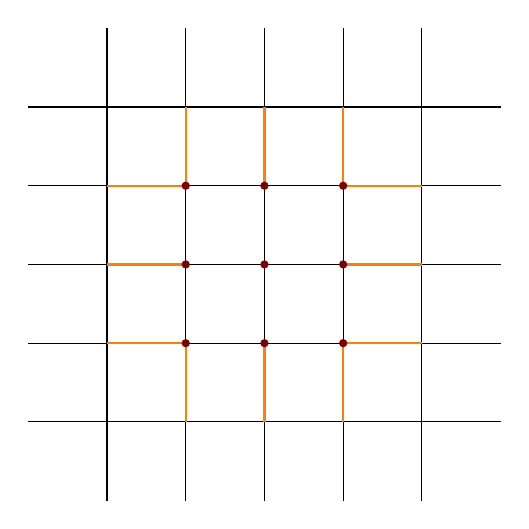
\begin{tikzpicture}
          \foreach \x in {-2, -1, 0, 1, 2} {
             \draw (\x, -3) -- (\x, 3);
             \draw (-3, \x) -- (3, \x);
          }
          \foreach \x in {-1, 0, 1} {
            \draw [morange, thick] (1, \x) -- (2, \x);
            \draw [morange, thick] (-1, \x) -- (-2, \x);
            \draw [morange, thick] (\x, 1) -- (\x, 2);
            \draw [morange, thick] (\x, -1) -- (\x, -2);
          }
          \foreach \x in {-1, 0, 1} {
             \foreach \y in {-1, 0, 1} {
               \node [circ, mred] at (\x, \y) {};
            }
          }
        \end{tikzpicture}
      \end{center}
      Then if $A$ consists of the red points, then the boundary consists of the orange edges.

      Then $\Gamma$ is non-amenable iff there exists $c (s, \Gamma) > 0$ such that for all $A \subseteq \Gamma$, we have $|\partial A| \geq c|A|$.
    \item There exists infinite, finitely generated, simple, anemable groups.
    \item If $\Gamma \subseteq \GL(n, \C)$, then $\Gamma$ is amenable iff it contains a finite-index subgroup which is solvable.
    \item $\Free_2$ is non-amenable.
    \item Any non-elementary word-hyperbolic group is non-amenable.
  \end{itemize}
\end{eg}

So quite a few groups are non-amenable. Which is good, because now the following vanishing theorem would not apply!

\begin{prop}
  Let $\Gamma$ be an amenable group. Then $H^k_b(\Gamma, \R) = 0$ for $k \geq 1$.
\end{prop}

The proof requires absolutely no idea.
\begin{proof}
  Let $k \geq 1$ and $f: \Gamma^{k + 1} \to \R$ a $\Gamma$-invariant bounded cocycle. In other words,
  \begin{align*}
    d^{(k + 1)} f &= 0\\
    f(\gamma\gamma_0, \cdots, \gamma\gamma_k) &= f(\gamma_0, \cdots, \gamma_k).
  \end{align*}
  We have to find $\varphi: \Gamma^k \to \R$ bounded such that
  \begin{align*}
    d^{(k)} \varphi &= f\\
    \varphi(\gamma\gamma_0, \cdots, \gamma\gamma_{k - 1}) &= \varphi(\gamma_0, \cdots, \gamma_{k - 1}).
  \end{align*}
  Recall that for $\eta \in \Gamma$, we can define
  \[
    h_\eta (\gamma_0, \cdots, \gamma_{k - 1}) = (-1)^{k + 1} f(\gamma_0, \cdots, \gamma_{k + 1}, \eta),
  \]
  and then
  \[
    d^{(k + 1)}f = 0 \Longleftrightarrow f = d^{(k)}(h_\eta).
  \]
  However, $h_\eta$ need not be invariant. Instead, we have
  \[
    h_\eta(\gamma\gamma_0, \cdots, \gamma\gamma_{k - 1}) = h_{\gamma^{-1} \eta} (\gamma_0, \cdots, \gamma_{k - 1}).
  \]
  Now let $m : \ell^\infty(\Gamma) \to \R$ be a left-invariant mean. We notice that the map
  \[
    \eta \mapsto h_\eta (\gamma_0, \cdots, \gamma_{k - 1})
  \]
  is bounded by $\|f\|_\infty$. So we can define
  \[
    \varphi(\gamma_0, \cdots, \gamma_{k - 1}) = m \Big\{ \eta \mapsto h_\eta (\gamma_0, \cdots, \gamma_{k - 1})\Big\}.
  \]
  Then this is the $\varphi$ we want. Indeed, we have
  \[
    \varphi(\gamma \gamma_0, \cdots, \gamma \gamma_{k - 1}) = m \Big\{ \eta \mapsto h_{\gamma^{-1}\eta} (\gamma_0, \cdots, \gamma_{k - 1})\Big\}.
  \]
  But this is just the mean of a left translation of the original function. So this is just $\varphi(\gamma_0, \cdots, \gamma_{k - 1}$. Also, by properties of the mean, we know $\|\varphi\|_\infty \leq \|f\|_\infty$.

  Finally, by linearity, we have
  \begin{align*}
    d^{(k)} \varphi(\gamma_0, \cdots, \gamma_k) &= m \Big\{ \eta \mapsto d^{(k)} h_\eta (\gamma_0, \cdots, \gamma_k) \Big\}\\
    &= m \Big\{ f(\gamma_0, \cdots, \gamma_k) \cdot \mathbf{1}_\Gamma\Big\}\\
    &= f(\gamma_0, \cdots, \gamma_k) m (\mathbf{1}_\Gamma)\\
    &= f(\gamma_0, \cdots, \gamma_k).
  \end{align*}
\end{proof}

\section{Actions on \tph{$S^1$}{S1}{S<sup>1</sup>}}
\subsection{The bounded Euler class}
We are now going to focus our study on actions on $S^1$. Recall that the central extension
\[
  \begin{tikzcd}
    0 \ar[r] & \Z \ar[r] & \Homeo^+_\Z(\R) \ar[r] & \Homeo^+(S^1) \ar[r] & 0
  \end{tikzcd}
\]
defines the Euler class $e \in H^2(\Homeo^+(S^1), \Z)$. We have also shown that there is a representative cocycle $c(f, g)$ taking the values $\{0, 1\}$, defined by
\[
  \overline{f \circ g} \circ T_{c(f, g)} = \bar{f} \circ \bar{g},
\]
where for any $f$, the map $\bar{f}$ is the unique lift to $\R$ such that $\bar{f}(0) = [0, 1)$.

Since $c$ takes values in $\{0, 1\}$, in particular, it is a bounded cocycle. So we can use it to define
\begin{defi}[Bounded Euler class]\index{bounded Euler class}\index{Euler class!bounded}\index{$e^b$}
  The \emph{bounded Euler class}
  \[
    e^b \in H_b^2(\Homeo^+(S^1), \Z)
  \]
  is the bounded cohomology class represented by the cocycle $c$.
\end{defi}

By construction, $e^b$ is sent to $e$ via the comparison map
\[
  \begin{tikzcd}
    c_2: H_b^2(\Homeo^+(S^1), \Z) \ar[r] & H^2(\Homeo^+(S^1), \Z)
  \end{tikzcd}.
\]
In fact, the comparison map is injective. So this $e^b$ is the unique element that is sent to $e$, and doesn't depend on us arbitrarily choosing $c$ as the representative.

\begin{defi}[Bounded Euler class of action]\index{bounded Euler class}\index{Euler class!bounded}
  The bounded Euler class of an action $h: \Gamma \to \Homeo^+(S^1)$ is $h^*(e^b) \in H_b^2(\Gamma, \Z)$.
\end{defi}

By naturality (proof as exercise), $h^*(e^b)$ maps to $h^*(e)$ under the comparison map. The following is also an exercise:

\begin{ex}
  Show that if $h: \Z \to \Homeo^+(S^1)$ and $\varphi = h(1)$, then under the isomorphism
  \[
    H^2_b(\Z, \Z) \to \R/\Z,
  \]
  we have $h^*(e^b) = \Rot(\varphi)$, the Poincar\'e rotation number of $\varphi$.
\end{ex} % prove this

So this tells us the bounded Euler class is a natural generalization of the Poincar\'e rotation number.

\begin{ex}
  Assume $h: \Gamma \to \Homeo^+(S^1)$ takes values in the rotations $\Rot$. Let $\chi: \Gamma \to \R/\Z$ the corresponding homomorphism. Then under the connecting homomorphism
  \[
    \begin{tikzcd}
      \Hom(\Gamma, \R/\Z) \ar[r, "\delta"] & H_b^2(\Gamma, \Z)
    \end{tikzcd},
  \]
  we have $\delta(\chi) = h^*(e^b)$.
\end{ex}

\begin{ex}
  If $h_1$ and $h_2$ are conjugate in $\Homeo^+(S^1)$, i.e.\ there exists a $\varphi \in \Homeo^+(S^1)$ such that $h_1(\gamma) = \varphi h_2(\gamma) \varphi^{-1}$, then
  \[
    h_1^*(e) = h_2^*(e),\quad h_1^*(e^b) = h_2^*(e^b).
  \]
  The proof involves writing out a lot of terms explicitly.
\end{ex}

How powerful is this bounded Euler class in distinguishing actions? We saw that conjugate actions have the same bounded Euler class. The converse does not hold. One can show that any action with a global fixed point has trivial bounded Euler class, and there are certainly non-conjugate actions that both have global fixed points (e.g. take one of them to be the trivial action).

It turns out there is a way to extend the notion of conjugacy so that the bounded Euler class becomes a complete invariant.

\begin{defi}[Increasing map of degree $1$]\index{increasing map}\index{increasing map!degree 1}
  A map $\varphi: S^1 \to S^1$ is \emph{increasing of degree $1$} if there is some $\tilde{\varphi}: \R \to \R$ lifting $\varphi$ such that $\tilde{\varphi}$ is is monotonically increasing and
  \[
    \tilde{\varphi}(x + 1) = \tilde{\varphi}(x) + 1
  \]
  for all $x \in \R$.
\end{defi}
Note that there is no continuity assumption made on $\varphi$. On the other hand, it is an easy exercise to see that any monotonic map $\R \to \R$ has a countable set of discontinuities. This is also not necessarily injective.

\begin{eg}
  The constant map $S^1 \to S^1$ sending $x \to 0$ is increasing of degree $1$, as it has a lift $\tilde{\varphi}(x) = [x]$.
\end{eg}

Equivalently, such a map is one that sends a positive $4$-tuple to a weakly positive $4$-tuple (exercise!). % picture and explain

\begin{defi}[Semiconjugate action]\index{semiconjugate action}\index{action!semiconjugate}\index{conjugate!semi-}
  Two actions $h_1, h_2: \Gamma \to \Homeo^+(S^1)$ are semi-conjugate if there are increasing maps of degree $1$ $\varphi_1, \varphi_2: S^1 \to S^1$ such that
  \begin{enumerate}
    \item $h_1(\gamma) \varphi_1 = \varphi_1 h_2(\gamma)$ for all $\gamma \in \Gamma$;
    \item $h_2(\gamma) \varphi_2 = \varphi_2 h_1(\gamma)$ for all $\gamma \in \Gamma$.
  \end{enumerate}
\end{defi}
One can check that the identity action is semiconjugate to any action with a global fixed point.

Recall the following definition:
\begin{defi}[Minimal action]\index{minimal action}\index{action!minimal}
  An action on $S^1$ is \emph{minimal} if every orbit is dense.
\end{defi}

\begin{lemma}
  If $h_1$ and $h_2$ are minimal actions that are semiconjugate via $\varphi_1$ and $\varphi_2$, then $\varphi_1$ and $\varphi_2$ are homeomorphisms and are inverses of each other.
\end{lemma}

\begin{proof}
  The condition (i) tells us that
  \[
    h_1(\gamma) (\varphi_1(x)) = \varphi_1(h_2(\gamma)(x)).
  \]
  for all $x \in S^1$ and $\gamma \in \Gamma$. This means $\im \varphi_1$ is $h_1(\Gamma)$-invariant, hence dense in $S^1$. Thus, we know that $\im \tilde{\varphi}_1$ is dense in $\R$. But $\tilde{\varphi}$ is increasing. So $\tilde{\varphi}_1$ must be continuous. Indeed, we can look at the two limits
  \[
    \lim_{x \nearrow y} \tilde{\varphi}_1(x) \leq \lim_{x \searrow y} \tilde{\varphi}_1(x).
  \]
  But since $\tilde{\varphi}_1$ is increasing, if $\tilde{\varphi}_1$ were discontinuous at $y \in \R$, then the inequality would be strict, and hence the image misses a non-trivial interval. So $\tilde{\varphi}_1$ is continuous.

  We next claim that $\tilde{\varphi}_1$ is injective. Suppose not. Say $\varphi(x_1) = \varphi(x_2)$. Then by looking at the lift, we deduce that $\varphi((x_1, x_2)) = \{x\}$ for some $x$. Then by minimality, it follows that $\varphi$ is locally constant, hence constant, which is absurd.

  We can continue on and then decide that $\varphi_1, \varphi_2$ are homeomorphisms. % complete
\end{proof}

\begin{thm}[F. Ghys, 1984]
  Two actions $h_1$ and $h_2$ are semiconjugate iff $h_1^*(e^b) = h_2^*(e^b)$.
\end{thm}
Thus, in the case of minimal actions, the bounded Euler class is a complete invariant of actions up to conjugacy.

\begin{proof}
  We shall only prove one direction, that if the bounded Euler classes agree, then the actions are semi-conjugate.

  Let $h_1, h_2: \Gamma \to \Homeo^+(S^1)$. Recall that $c(f, g) \in \{0, 1\}$ refers to the (normalized) cocycle defining the bounded Euler class. Therefore
  \begin{align*}
    c_1(\gamma, \eta) &= c(h_1(\gamma), h_1(\eta))\\
    c_2(\gamma, \eta) &= c(h_2(\gamma), h_2(\eta)).
  \end{align*}
  are representative cocycles of $h_1^*(e^b), h_2^*(e^b) \in H_b^2(\Gamma, \Z)$.

  By the hypothesis, there exists $u: \Gamma \to \Z$ bounded such that
  \[
    c_2(\gamma, \eta) = c_1(\gamma, \eta) + u(\gamma) - u(\gamma\eta) + u(\eta)
  \]
  for all $\gamma, \eta \in \Gamma$.

  Let $\bar{\Gamma} = \Gamma \times_{c_1} \times \Z$ be constructed with $c_1$, with group law
  \[
    (\gamma, n)(\eta, m) = (\gamma \eta, c_1(\gamma, \eta) + n + m)
  \]
  We have a section
  \begin{align*}
    s_1: \Gamma &\to \bar{\Gamma} \\
    \gamma &\mapsto (\gamma, 0).
  \end{align*}
  We also write $\delta = (e, 1) \in \bar{\Gamma}$, which generates the copy of $\Z$ in $\bar{\Gamma}$. Then we have
  \[
    s_1(\gamma \eta) \delta^{c_1(\gamma, \eta)} = s_1(\gamma) s_2(\eta).
  \]
  Likewise, we can define a section by
  \[
    s_2(\gamma) = s_1(\gamma) \delta^{u(\gamma)}.
  \]
  Then we have
  \begin{align*}
    s_2(\gamma \eta) &= s_1 (\gamma \eta) \delta^{u(\gamma \eta)} \\
    &= \delta^{-c_1(\gamma, \eta)} s_1(\gamma) s_1 (\eta) \delta^{u(\gamma \eta)}\\
    &= \delta^{-c_1(\gamma, \eta)} \delta^{-u(\gamma)} s_2(\gamma) \delta^{-u(\eta)} s_2 (\eta) \delta^{u(\gamma \eta)}\\
    &= \delta^{-c_1(\gamma, \eta) - u(\gamma) + u(\gamma \eta) - u(\eta)} s_2 (\gamma) s_2(\eta)\\
    &= \delta^{-c_2(\gamma, \eta)} s_2(\gamma) s_2(\eta).
  \end{align*}
  Now every element in $\bar{\Gamma}$ can be uniuely written as a product $s_1(\gamma) \delta^n$, and the same holds for $s_2(\gamma) \delta^m$.

  Recall that for $f \in \Homeo^+(S^1)$, we write $\bar{f}$ for the unique lift with $\bar{f}(0) \in [0, 1)$. We define
  \[
    \Phi_i (s_i(\gamma) \delta^n) = \overline{h_i(\gamma)} \cdot T_n.
  \]
  We claim that this is a homomorphism! We simply compute
  \begin{align*}
    \Phi_i (s_i(\gamma) \delta^n s_i(\eta) \delta^m) &= \Phi_i(s_i(\gamma) s_i(\eta) \delta^{n + m})\\
    &= \Phi_i(s_i(\gamma \eta) \delta^{c_i(\gamma, \eta) + n + m})\\
    &= \overline{h_i(\gamma \eta)} T_{c_i(\gamma, \eta)} T_{n + m}\\
    &= \overline{h}_i(\gamma) \overline{h}_i(\eta) T_{n + m}\\
    &= \overline{h}_i(\gamma) T_n \overline{h}_i(\eta) T_m\\
    &= \Phi_i(s_i(\gamma) \delta^n) \Phi_i(s_i(\eta) \delta^m).
  \end{align*}
  So we get group homomorphisms $\Phi_i: \bar{\Gamma} \to \Homeo^+_\Z(\R)$.

  \begin{claim}
    For any $x \in \R$, the map
    \begin{align*}
      \bar{\Gamma} &\to \R\\
      g &\mapsto \Phi_1(g)^{-1} \Phi_2(g) (x)
    \end{align*}
    is bounded.
  \end{claim}

  \begin{proof}
    We define
    \[
      v(g, x) = \Phi_1(g)^{-1} \Phi(g)x.
    \]
    We notice that
    \begin{align*}
      v(g \delta^m, x) &= \Phi_1(g \delta^m)^{-1} \Phi_2(g \delta^m)(x)\\
      &= \Phi_1(g)^{-1} T_{-m} T_m \Phi_2(g)\\
      &= v(g, x).
    \end{align*}
    Also, for all $g$, the map $x \mapsto v(g, x)$ is in $\Homeo^+_\Z(\R)$.

    Hence it is sufficient to show that
    \[
      \gamma \mapsto v(s_2(\gamma), 0)
    \]
    is bounded. Indeed, we just have
    \begin{align*}
      v(s_2(\gamma), 0) &= \Phi_1 (s_2(\gamma)^{-1} \Phi_2(s_2(\gamma))(0)\\
      &= \Phi_1(s_1(\gamma) \delta^{u(\gamma)})^{-1} \Phi_2(s_2(\gamma))(0)\\
      &= \delta^{-u(\gamma)} \overline{h_1(\gamma)}^{-1} \overline{h_2(\gamma)} (0)\\
      &= - u(\gamma) + \overline{h_1(\gamma)}^{-1} (\overline{h_2}(\gamma)(0)).
    \end{align*}
    But $u$ is bounded, and also
    \[
      \overline{h_1(\gamma)}^{-1} (\overline{h_2(\gamma)}(0)) \in (-1, 1).
    \]
    So we are done.
  \end{proof}
  Finally, we can write down our two quasi-conjugations. We define
  \[
    \tilde{\varphi}(x) = \sup_{g \in \bar{\Gamma}} v(g, x).
  \]
  Then we verify that
  \[
    \tilde{\varphi}(\Phi_2(h) x) = \Phi_1(h)(\varphi(x)).
  \]
  Reducing everything modulo $\Z$, we find that
  \[
    \varphi h_2(\gamma) = h_1(\gamma) \varphi.
  \]
  The other direction is symmetric.
\end{proof}

\subsection{The real bounded Euler class}
\begin{defi}[Real bounded Euler class]\index{real bounded Euler class}\index{bounded Euler class!real}\index{Euler class!real bounded}
  The \emph{real bounded Euler class} is the class $e_\R^b \in H_b^2(\Homeo^+(S^1), \R)$ obtained by change of coefficients from $\Z \to \R$.

  The real bounded Euler class of an action $h: \Gamma \to \Homeo^+(S^1)$ is the pullback
  \[
    h^*(e_\R^b) \in H_b^2(\Gamma, \R).
  \]
\end{defi}

Hence, $e^b_\R$ is the image under the morphism induced by $\Z \to \R$ in cohomology of $e^b \in H_b^2(\Homeo^+(S^1), \Z)$.

A priori, this class contains less information that the original Euler class. However, the vanishing or non-vanishing of $h^*(e^b_\R)$ distinguishes between very different dynamical properties.

\begin{cor}
  An action $h$ is semi-conjugate to an action by rotations iff $h^*(e_\R^b) = 0$.
\end{cor}

\begin{proof}\leavevmode
  \begin{itemize}
    \item[($\Rightarrow$)] Let $h_1: \Gamma \to \Rot \subseteq \Homeo^+(S^1)$ be semi-conjugate to $h$. Let $\chi: \Gamma \to \R/\Z$ be the associated group homomorphism under the isomorphism $\Rot \cong \R/\Z$. Recall from a previous exercise that
      \[
        h_1^*(e^b) = \delta(\chi),
      \]
      where $\delta$ is the connecting homomorphism in
      \[
        \begin{tikzcd}
          0 \ar[r] & \Hom(\Gamma, \R/\Z) \ar[r, "\delta"] & H_b^2(\Gamma, \Z) \to H_b^2(\Gamma, \R)
        \end{tikzcd}.
      \]
      So $h^*(e^b) = h_1^*(e^b) = \delta(\chi)$. But by exactness, the image in $H_b^2(\Gamma, \R)$ vanishes.

    \item[($\Leftarrow$)] Suppose $h^*(e_\R^b) = 1$. Then $h^*(e^b) \in H_b^2(\Gamma, \Z)$ is in the kernel of the map $H^2_b(\Gamma, \Z) \to H^2_b(\Gamma, \R)$. Hence, by exactness, there exists $\chi \in \Hom(\Gamma, \R/\Z)$ such that $\delta(\chi) = h^*(e^b_\R)$. Then we can define $h_1: \Gamma \to \Rot$ to be given by $\chi$. Then $h_1^*(e^b) = \delta(\chi) = h(e^b)$. So $h$ is semi-conjugate to $h_1$.
  \end{itemize}
\end{proof}

We want to use the real bounded Euler class to classify different kinds of actions. To do so, we need the following trichotomy concerning actions on $S^1$. More details can be found in Hector--Hirsch's \emph{Introduction to the geometry of foliations}.

\begin{thm}
  Let $h: \Gamma \to \Homeo^+(S^1)$ be an action. Then one of the following holds:
  \begin{enumerate}
    \item There is a finite orbit, and all finite orbits have the same cardinality.
    \item The action is minimal.
    \item There is a closed, minimal, invariant, infinite, proper subset $K \subsetneq S^1$ such that any $x \in S^1$, the closure of the orbit $\overline{h(\Gamma) x}$ contains $K$.
  \end{enumerate}
\end{thm}

\begin{proof}[Proof sketch]
  First one uses compactness and Zorn's lemma to show the existence of minimal, non-empty, closed, invariant subsets.

  Let $K \subseteq S'$ be such a subset, and let $\partial K = K \setminus \mathring{K}$. We let $K'$ be the set of all accumulation points of $K$ (i.e.\ the set of all points $x$ such that every neighbourhood of $x$ contains infinitely many points of $K$). Clearly $K'$ and $\partial K$ are closed and invariant as well, and contained in $K$. By minimality, they must be $K$ or empty.

  \begin{enumerate}
    \item If $K' = \emptyset$, then $K$ is finite. It is an exercise to show that all orbits have the same size.
    \item If $K' = K$, and $\partial K = \emptyset$, then $K = \mathring{K}$, and hence is open. Since $S^1$ is connected, $K = S^1$, and the action is minimal.
    \item If $K' = K = \partial K$, then $K$ is \emph{perfect}, i.e.\ every point is an accumulation point, and $K$ is totally disconnected. We definitely have $K \not= S^1$ and $K$ is infinite. It is also minimal and invariant.

      Let $x \in S^1$. If it is in $K$, then the closure of its orbit is certainly contained in $K$. If $x \not\in K$, then $S^1 \setminus K$ is a disjoint (countable) union of open intervals. More precisely, if $a, b \in S^1$ and $a \not= b$, then an open interval is\index{open interval!of circle}
      \[
        (a, b) = \{z \in S^1: (a, z, b)\text{ is positively oriented}\}.
      \]
      Now let $(a, b)$ be the connected component of $S^1 \setminus K$ containing $x$.

      Since $h(\Gamma)a$ consists of end points of open intervals, it must be countable. But since $K$ is perfect, it is not countable. So $K \setminus h(\Gamma) a$ is non-empty, hence dense in $K$. So it suffices to approximate any $y \in K \setminus h(\Gamma) a$.

      Now observe that $a \in K$. Hence by minimality, there exists a sequence $(\gamma_n)_{n \geq 1}$ such that $h(\gamma_n) a \to y$. But since $y \not \in h(\Gamma) a$, we may wlog that all the points $\{h(\gamma_n)a : n \geq 1\}$ are distinct. Hence $\{h(\gamma_n)(a, b) \}_{n \geq 1}$ is a collection of disjoint intervals in $S^1$. Hence their lengths tend to $0$. And then we are done, because then $h(\gamma_n) x$ gets arbitrarily close to $h(\gamma_n) a$ as well.
  \end{enumerate}
\end{proof}

\begin{cor}
  Let $h: \Gamma \to S^1$ be an action. Then one of the following is true:
  \begin{enumerate}
    \item $h^*(e^b_\R) = 0$ and $h$ is semi-conjugate to an action by rotations.
    \item $h^*(e^b_\R) \not= 0$, and then $h$ is semi-conjugate to a minimal \emph{unbounded}\index{unbounded action}\index{action!unbounded} action, i.e.\ $\{h(\gamma): \gamma \in \Gamma\}$ is not equicontinuous.
  \end{enumerate}
\end{cor}
Observe that if $\Lambda \subseteq \Homeo^+(S^1)$ is equicontinuous, then by Arzela--Ascoli, its closure $\bar{\Lambda}$ is compact.

\begin{lemma}
  A compact subgroup $U \subseteq \Homeo^+(S^1)$ is conjugate to a subgroup of $\Rot$.
\end{lemma}

\begin{proof}
  We shall assume $U$ is minimal, since that is what we care about. By Kakutani fixed point theorem, we can pick an $U$-invariant probability measure on $S^1$, say $\mu$ such that $\mu(S^1) = 2\pi$.

  We parametrize the circle by $p: [0, 2\pi) \to S^1$. We define
  \[
    \varphi(p(t)) = p(s),
  \]
  where $s \in [0, 2\pi)$ is unique with the property that
  \[
    \mu(p([0, s)) = t.
  \]
  One then verifies that $\varphi$ is a homeomorphism, and $\varphi U \varphi^{-1} \subseteq \Rot$.
\end{proof}

\begin{proof}[Proof of corollary]
  Suppose $h^*(e^b_\R) \not= 0$. Thus we are in case (ii) or (iii) of the trichotomy.

  We first show how to reduce (iii) to (ii). Let $K \subsetneq S^1$ be the minimal $h(\Gamma)$-invariant closed set given by the trichotomy theorem. The idea is that this $K$ misses a lot of open intervals, and we want to collapse those intervals.

  We define the equivalence relation on $S^1$ by $x \sim y$ if $\{x, y\} \subseteq \bar{I}$ for some connected component $I$ of $S^1 \setminus K$. Then $\sim$ is an equivalence relation that is $h(\Gamma)$-invariant, and the quotient map is homeomorphic to $S^1$ (exercise!). Write $i: S^1/\sim \to S^1$ for the isomorphism.

  In this way, we obtain an action of $\rho: \Gamma \to \Homeo^+(S^1)$ which is minimal, and the map
  \[
    \varphi:
    \begin{tikzcd}
      S^1 \ar[r, "\mathrm{pr}"] & S^1/\sim \ar[r, "i"] & S^1
    \end{tikzcd}
  \]
  intertwines the two actions, i.e.
  \[
    \varphi h(\gamma) = \rho(\gamma) \varphi.
  \]
  Then one shows that $\varphi$ is increasing of degree $1$. Then we would need to find $\psi: S^1 \to S^1$ which is increasing of degree $1$ with
  \[
    \psi \rho(\gamma) = h(\gamma) \psi.
  \]
  But $\varphi$ is surjective, and picking an appropriate section of this would give the $\psi$ desired.

  So $h$ is semi-conjugate to $\rho$, and $0 \not= h^*(e^b_\R) = \rho^*(e^b_\R)$.

  Thus we are left with $\rho$ minimal, with $\rho^*(e^b_\R) \not= 0$. We have to show that $\rho$ is not equicontinuous. But if it were, then $\rho(\Gamma)$ would be contained in a compact subgroup of $\Homeo^+(S^1)$, and hence by the previous lemma, would be conjugate to an action by rotation.
\end{proof}

The following theorem gives us a glimpse of what unbounded actions look like:
\begin{thm}[Ghys, Margulis]
  If $\rho: \Gamma \to \Homeo^+(S^1)$ is an action which is minimal and unbounded. Then the centralizer $C_{\Homeo^+(S^1)}(\rho(\Gamma))$ is finite cyclic, say $\bra \varphi\ket$, and the factor action $\rho_0$ on $S^1/\bra \varphi\ket \cong S^1$ is minimal and strongly proximal. We call this action the \term{strongly proximal quotient} of $\rho$.
\end{thm}

\begin{defi}[Strongly proximal action]\index{strongly proximal action}\index{action!strongly proximal}
  A $\Gamma$-action by homeomorphisms on a compact metrizable space $X$ is \emph{strongly proximal} if for all probability measures $\mu$ on $X$, the weak-$*$ closure $\overline{\Gamma}_* \mu$ contains a Dirac mass.
\end{defi}

For a minimal action on $X = S^1$, the property is equivalent to the following:
\begin{itemize}
  \item Every proper closed interval can be contracted. In other words, for every interval $J \subseteq S^1$, there exists a sequence $(\gamma_n)_{n \geq 1}$ such that $\diam(\rho(\gamma_n)J) \to 0$ as $n \to \infty$.
\end{itemize}

\begin{proof}[Proof of theorem]
  Let $\psi$ commute with all $\rho(\gamma)$ for all $\gamma \in \Gamma$, and assume $\psi \not= \id$.
  \begin{claim}
    $\psi$ has no fixed points.
  \end{claim}

  \begin{proof}
    Otherwise, if $\psi(p) = p$, then
    \[
      \psi(\rho(\gamma) p) = \rho(\gamma) \psi(p) = \rho(\gamma)(p).
    \]
    Then by density of $\{\rho(\gamma) p: \gamma \in \Gamma\}$, we have $\psi = \id$.
  \end{proof}

  Hence we can find $\varepsilon > 0$ such that $\length([x, \psi(x)]) \geq \varepsilon$ for all $x$ by compactness. Observe that
  \[
    \rho(\gamma) [x, \psi(x)] = [\rho(\gamma) x, \rho(\gamma) \psi(x)] = [\rho(\gamma) x, \psi(\rho(\gamma)x)].
  \]
  This is just an element of the above kind. So $\length(\rho(\gamma)[x, \psi(x)]) \geq \varepsilon$.

  Now assume $\rho(\Gamma)$ is minimal and not equicontinuous.
  \begin{claim}
    Every point $x \in S^1$ has a neighbourhood that can be contracted.
  \end{claim}

  \begin{proof}
    Indeed, since $\rho(\Gamma)$ is not equicontinuous, there exists $\varepsilon > 0$, a sequence $(\gamma_n)_{n \geq 1}$ and intervals $I_k$ such that $\length(I_k) \searrow 0$ and $\length(\rho(\gamma_n)I_n) \geq \varepsilon$.

    Since we are on a compact space, after passing to a subsequence, we may assume that for $n$ large enough, we can find some interval $J$ such that $\length(J) \geq \frac{\varepsilon}{2}$ and $J \subseteq \rho(\gamma_n) I_n$.

    But this means
    \[
      \rho(\gamma_n)^{-1} J \subseteq I_n.
    \]
    So $J$ can be contracted. Since the action is minimal,
    \[
      \bigcup_{\gamma \in \Gamma} \rho(\gamma) J = S^1.
    \]
    So every point in $S^1$ is contained in some interval that can be contracted.
  \end{proof}

  We shall now write down what the homeomorphism that generates the centralizer. Fix $x \in S^1$. Then the set
  \[
    \mathcal{C}_x = \{[x, y) \in S^1: [x, y)\text{ can be contracted}\}
  \]
  is totally ordered ordered by inclusion. Define
  \[
    \varphi(x) \sup \mathcal{C}_x.
  \]
  Then
  \[
    [x, \varphi(x)) = \bigcup \mathcal{C}_x.
  \]
  This gives a well-defined map $\varphi$ that commutes with the action of $\gamma$. It is then an interesting exercise to verify all the desired properties.
  \begin{itemize}
    \item To show $\varphi$ is homeomorphism, we show $\varphi$ is increasing of degree $1$, and since it commutes with a minimal action, it is a homeomorphism.

    \item If $\varphi$ is not periodic, then there is some $n$ such that $\varphi^n(x)$ is between $x$ and $\varphi(x)$. But since $\varphi$ commutes with the action of $\Gamma$, this implies $[x, \varphi^n(x)]$ cannot be contracted, which is a contradiction.
  \end{itemize}
\end{proof}

\begin{ex}
  We have
  \[
    \rho^*(e^b) = k \rho^*_0(e^b),
  \]
  where $k$ is the cardinality of the centralizer.
\end{ex}

\begin{eg}
  We can decompose $\PSL(2, \R) = \PSO(2) AN$, where
  \[
    A = \left\{
      \begin{pmatrix}
        \lambda & 0\\
        0 & \lambda^{-1}
      \end{pmatrix}: \lambda > 0
    \right\},\quad N = \left\{
      \begin{pmatrix}
        1 & x\\
        0 & 1
      \end{pmatrix}
    \right\}.
  \]
  More precisely, $SO(2) \times A \times N \to \SL(2, \R)$ is a diffeomorphism and induces on $\PSO(2)\times A \times N \to \PSL(2, \R)$. In particular, the inclusion $i: \PSO(2) \hookrightarrow \PSL(2, \R)$ induces an isomorphism on the level of $\pi_1 \cong \Z$.

  We can consider the subgroup $k\Z \subseteq \Z$. which gives us a covering of $\PSO(2)$ and $\PSL(2, \R)$ that fits in the diagram
  \[
    \begin{tikzcd}
      \PSO(2)_k \ar[r, "i_k"] \ar[d, "p"] & \PSL(2, \R) \ar[d, "p"]\\
      \PSO(2) \ar[r, "i"] & \PSL(2, \R)
    \end{tikzcd}.
  \]
  On the other hand, if we put $B = A \cdot N$, which is a contractible subgroup, we obtain a homomorphism $s: B \to \PSL(2, \R)_k$, and we find that
  \[
    \PSL(2, \R)_k \cong \PSO(2)_k \cdot s(B).
  \]
  So we have
  \[
    \frac{\PSL(2, \R)_k}{ s(B)} \cong \PSO(2)_k.
  \]
  So $\PSL(2, \R)_k/s(B)$ is homeomorphic to a circle. So we obtain an action of $\PSL(2, \R)_k$ on the circle. % homogeneous space

  Now we can think of $\Gamma \cong \Free_r$ as a lattice in $\PSL(2, \R)$. Take any section $\sigma: \Gamma \to \PSL(2, \R)_k$. This way, we obtain an unbounded minimal action with centralizer isomorphic to $\Z/k\Z$.
\end{eg}

\begin{defi}[Lattice]\index{lattice}
  A lattice in a locally compact group $G$ is a discrete subgroup $\Gamma$ such that on $\Gamma \backslash G$, there is a $G$-invariant probability measure.
\end{defi}

\begin{eg}
  Let $\mathcal{O}$ be the ring of integers of a finite extension $k/\Q$. Then $\SL(n, \mathcal{O})$ is a lattice in an appropriate Lie group. To construct this, we write $[k:\Q] = r + 2s$, where $r$ and $2s$ are the number of real and complex field embeddings of $k$. Using these field embeddings, we obtain an injection
  \[
    \SL(n, \mathcal{O}) \to \SL(n, \R)^r \times \SL(n, \C)^s,
  \]
  and the image is a lattice.
\end{eg}

\begin{eg}
  If $X$ is a complete proper CAT(0) space, then $\Isom(X)$ is locally compact, and in many cases conatins lattices.
\end{eg}

\begin{thm}[Burger, 2007]
  Let $G$ be a second-countable locally compact group, and $\Gamma < G$ be a lattice, and $\rho: \Gamma \to \Homeo^+(S^1)$ a minimal unbounded action. Then the following are equivalent:
  \begin{itemize}
    \item $\rho^*(e^b_\R)$ is in the image of the restriction map $H^2_{bc}(G, \R) \to H_b^2(\Gamma, \R)$ % bc is continuous
    \item The strongly proximal quotient $\rho_{ss}: \Gamma \to \Homeo^+(S^1)$ extends continuously to $G$. % introduce _ss notation for strongly proximal quotient.
  \end{itemize}
\end{thm}
% ``an extension criterion for lattice actions on the circle'' in ``Geometry, rigidity, and group actions'', Chicago

\begin{thm}[Burger--Monod, 2002]
  The restriction map $H^2_{bc}(G) \to H^2_b(\Gamma, \R)$ is an isomorphism in the following cases:
  \begin{enumerate}
    \item $G = G_1 \times \cdots \times G_n$ is a cartesian product of locally compact groups and $\Gamma$ has dense projections on each individual factor.
    \item $G$ is a connected semisimple Lie group with finite center and rank $G \geq 2$, and $\Gamma$ is irreducible.
  \end{enumerate}
\end{thm}

\begin{eg}
  Let $k/\Q$ be a finite extension that is not an imaginary quadratic extension. Then we have an inclusion
  \[
    \SL(2, \mathcal{O}) \hookrightarrow \SL(2, \R)^r \times \SL(2, \C)^s
  \]
  and is a product of more than one thing. One can actually explicitly compute the continuous bounded cohomology group of the right hand side.
\end{eg}

\begin{ex}
  Let $\Gamma < \SL(3, \R)$ be any lattice. Are tehre any actions by oriented homeomorphisms on $S^1$?

  Let's discuss according to $\rho^*(e^b_\R)$.
  \begin{itemize}
    \item If $\rho^*(e^b_\R) = 0$, then there is a finite orbit. Then we are stuck, and don't know what to say.
    \item If $\rho^*(e^b_\R) \not= 0$, then we have an unbounded minimal action. This leads to a strongly proximal action $\rho_{ss}: \Gamma \to \Homeo^+(S^1)$. But by the above results, this implies the action extends continuously to an action of $\SL(3, \R)$ on $S^1$. But $\SL(3, \R)$ contains $\SO(3)$, which is a compact group. But we know what compact subgroups of $\Homeo^+(S^1)$ look like, and it eventually follows that the action is trivial. So this case is not possible.
  \end{itemize}
\end{ex}

We say a topological group $T$ has \emph{small subgroups} if every neighbourhood of the identity contains a non-trivial subgroup. Typical examples include $(\Z/2\Z)^\N$, under the product topology.

\section{The relative homological approach}
\subsection{Injective modules}
When we defined ordinary group cohomology, we essentially defined it as the right-derived functor of taking invariants. While we do not need the machinery of homological algebra and derived functors to define group cohomology, having that available means we can pick different injective resolutions to compute group cohomology depending on the scenario, and often this can be helpful. It also allows us to extend group cohomology to allow non-trivial coefficients. Thus, we would like to develop a similar theory for bounded cohomology.

We begin by specifying the category we are working over.
\begin{defi}[Banach $\Gamma$ module]\index{Banach $\Gamma$-module}\index{$\Gamma$-module!Banach}
  A Banach $\Gamma$-module is a Banach space $V$ together with an action $\Gamma \times V \to V$ by linear isometries.
\end{defi}
Given a Banach $\Gamma$-module $V$, we can take the submodule of $\Gamma$-invariants $V^\Gamma$. The relative homological approach tells us we can compute the bounded cohomology $H_b^\Cdot(\Gamma, \R)$ by first taking an appropriate exact sequences of Banach $\Gamma$-modules
\[
  \begin{tikzcd}
    0 \ar[r] & \R \ar[r, "d^{(0)}"] & E_0 \ar[r, "d^{(1)}"] & E_1 \ar[r, "d^{(2)}"] \ar[r] & \cdots,
  \end{tikzcd}
\]
and then take the cohomology of the complex of $\Gamma$-invariants
\[
  \begin{tikzcd}
    0 \ar[r] & E_0^\Gamma \ar[r, "d^{(1)}"] & E_1^\Gamma \ar[r, "d^{(2)}"] \ar[r] & E_2^\Gamma \ar[r] & \cdots
  \end{tikzcd}.
\]
Of course, this works if we take $E_k = C(\Gamma^{k + 1}, A)$ and $d^{(k)}$ to be the differentials we have previously constructed, since this is how we defined bounded cohomology. The point is that there exists a large class of ``appropriate'' exact sequences such that this procedure gives us the bounded cohomology.

We first need the following definition:
\begin{defi}[Admissible morphism]\index{admissible morphism}
  An injective morphism $i: A \to B$ of Banach spaces is \emph{admissible} if there exists $\sigma: B \to A$ with
  \begin{itemize}
    \item $\sigma i = \id_A$; and
    \item $\|\sigma\|\leq 1$.
  \end{itemize}
\end{defi}
This is a somewhat mysterious definition, but when we have such a situation, this in particular implies $\im A$ is closed and $B = i(A) \oplus \ker \sigma$. In usual homological algebra, we don't meet these kinds of things, because our vector spaces always have complements. However, here we need them.

\begin{defi}[Injective Banach $\Gamma$-module]\index{injective Banach $\Gamma$-module}\index{Banach $\Gamma$-module!injective}\index{$\Gamma$-module!injective Banach}
  A Banach $\Gamma$-module is injective if for any diagram
  \[
    \begin{tikzcd}
      A \ar[r, "i"] \ar[d, "\alpha"] & B\\
      E
    \end{tikzcd}
  \]
  where $i$ and $\alpha$ are morphisms of $\Gamma$-modules, and $i$ is injective admissible, then there exists $\beta : B \to E$ a morphism of $\Gamma$-modules such that
  \[
    \begin{tikzcd}
      A \ar[r, "i"] \ar[d, "\alpha"] & B \ar[ld, dashed, "\beta"]\\
      E
    \end{tikzcd}
  \]
  commutes and $\|\beta\| \leq \|\alpha\|$.
\end{defi}
In other words, we can extend any map from a closed complemented subspace of $B$ to $E$.

\begin{defi}[Injective resolution]\index{injective resolution}
  Let $V$ be a Banach $\Gamma$-module. An \emph{injective resolution} of $V$ is an exact sequence
  \[
    \begin{tikzcd}
      V \ar[r] & E_0 \ar[r] & E_1 \ar[r] & E_2 \ar[r] & \cdots
    \end{tikzcd}
  \]
  where each $E_k$ is injective.
\end{defi}
Then standard techniques from homological algebra imply the following theorem:
\begin{thm}
  Let $E^{\Cdot}$ be an injective resolution of $\R$ Then
  \[
    H^\Cdot(E^{\Cdot \Gamma}) \cong H_b^\Cdot(\Gamma, \R)
  \]
  as topological vector spaces.

  In case $E^\Cdot$ admits contracting homotopies, this isomorphism is semi-norm decreasing.
\end{thm}

Unsurprisingly, the defining complex for bounded cohomology were composed of injective $\Gamma$-modules.
\begin{lemma}\leavevmode
  \begin{itemize}
    \item $\ell^\infty(\Gamma^n)$ for $n \geq 1$ are all injective Banach $\Gamma$-modules.
    \item $\ell_{\mathrm{alt}}^\infty(\Gamma^n)$ for $n \geq 1$ are injective Banach $\Gamma$-modules as well.
  \end{itemize}
\end{lemma}
This is a verification. More interestingly, we have the following
\begin{prop}
  The trivial $\Gamma$-module $\R$ is injective iff $\Gamma$ is amenable.
\end{prop}
As an immediate corollary, we know that if $\Gamma$ is amenable, then all the higher bounded cohomology groups vanish, as $0 \to \R \to 0 \to 0 \to \cdots$ is an injective resolution.

\begin{proof}\leavevmode
  \begin{itemize}
    \item[$(\Rightarrow)$] Suppose $A$ is injective. Consider the diagram
      \[
        \begin{tikzcd}
          \R \ar[d, equals] \ar[r, "i"] & \ell^\infty(\Gamma)\\
          \R
        \end{tikzcd},
      \]
      where $i(t)$ is the constant function $t$. We need to verify that $i$ is an admissible injection. Then we see that $\sigma(f) = f(e)$ is a left inverse to $i$ and $\|\sigma\| \leq 1$. Then there exists a morphism $\beta: \ell^\infty(\Gamma) \to \R$ filling in the diagram with $\|\beta\| \leq \|\id_\R\| = 1$ and in particular
      \[
        \beta(\mathbf{1}_\Gamma) = 1
      \]
      Since the action of $\Gamma$ on $\R$ is trivial, this $\beta$ is an invariant linear form on $\Gamma$, and we see that this is an invariant mean.
    \item[$(\Leftarrow)$] Assume $\Gamma$ is amenable, and let $m: \ell^\infty(\Gamma) \to \R$ be an invariant mean. Consider a diagram
      \[
        \begin{tikzcd}
          A \ar[r, "i"] \ar[d, "\alpha"] & B\\
          \R
        \end{tikzcd}
      \]
      as in the definition of injectivity. Since $i$ is an admissible, it has a left inverse $\sigma: B \to A$. Then we can define
      \[
        \beta(v) = m \{\gamma \mapsto \alpha(\sigma(\gamma_* v))\}.
      \]
      Then this is an injective map $B \to \R$ and one can verify this works.
  \end{itemize}
\end{proof}

This theory allows us to study bounded cohomology with more general coefficients. This can also be extended to $G$ a locally-compact second-countable groups with coefficients a $G$-Banach module $E$ which is the dual of a continuous separable Banach module $E^b$. This is more technical and subtle, but it works.

\subsection{Amenable actions}
In Riemannian geometry, we have the Hodge decomposition theorem. It allows us to understand the de Rham cohomology of a Riemannian manifold in terms of the complex of harmonic forms, whose cohomology is the complex itself. In bounded cohomology, we don't have something like this, but we can produce a complex such that the complex is equal to the cohomology in the second degree.

The setting is that we have a locally-compact second-countable group $G$ with a non-singular action on a standard measure space $(S, \mathcal{M}, \mu)$. We require that the action map $G \times S \to S$ which is measurable. Moreover, for any $g \in G$, the measure $g_* \mu$ is equivalent to $\mu$. In other words, the $G$-action preserves the null sets.

\begin{eg}
  Let $M$ be a smooth manifold. Then the action of $\Diff(M)$ on $M$ is non-singular.
\end{eg}

We want to come up with a notion similar to amenability. This is what we call conditional expectation.
\begin{defi}[Conditional expectation]\index{conditional expectation}
  A \emph{conditional expectation} on $G \times S$ is a linear map $M: L^\infty(G \times S) \to L^\infty(S)$ such that
  \begin{enumerate}
    \item $M(1) = 1$;
    \item If $M \geq 0$, then $M(f) \geq 0$; and
    \item $M$ is $L^\infty(S)$-linear.
  \end{enumerate}
\end{defi}
We have a left $G$-action on $L^\infty(G \times S)$ given by the diagonal action, and also a natural on $L^\infty(S)$. We say $M$ is \term{$G$-equivariant} if it is $G$-equivariant.

\begin{defi}[Amenable action]\index{amenable action}\index{action!amenable}
  A $G$-action on $S$ is amenable if there exists a $G$-equivariant conditional expectation.
\end{defi}
Note that a point (with the trivial action) is a conditional $G$-space if $G$ is amenable itself.

\begin{eg}
  Let $H$ be a closed subgroup of $G$, then the $G$ action on $G/H$ is amenable iff $H$ is amenable.
\end{eg}

\begin{thm}[Burger--Monod, 2002]
  Let $G \times S \to S$ be a non-singular action. Then the following are equivalent:
  \begin{enumerate}
    \item The $G$ action is amenable.
    \item $L^\infty(S)$ is an injective $G$-module.
    \item $L^\infty(S^n)$ for all $n \geq 1$ is injective.
  \end{enumerate}
\end{thm}
So any amenable $G$-space can be used to compute the bounded cohomology of $G$.

\begin{cor}
  If $(S, \mu)$ is an amenable $G$-space, then we have an isometric isomorphism $H^\Cdot(L^\infty(S^n, \mu)^G, d_n) \cong H^\Cdot(L^\infty_{\mathrm{alt}}(S^n, \mu)^G, d_n) \cong H_b(G, \R)$.
\end{cor}

\begin{eg}
  Let $\Gamma < G$ be a lattice in $\SL(n, \R)$, say. Let $P < G$ be a parabolic subgroup, e.g. the subgroup of upper-triangular matrices. We use $L^\infty_{\mathrm{alt}} ((G/P)^n)^\Gamma$ to compute bounded cohomology of $\Gamma$, since the restriction of amenable actions to closed subgroups is amenable. We have
  \[
    \begin{tikzcd}[row sep=small]
      0 \ar[r] & L^\infty(G/p)^\Gamma \ar[r] \ar[d, equals] & L_{\mathrm{alt}} ((G/P)^2)^\Gamma \ar[r] \ar[d, equals] & L_{\mathrm{alt}} ((G/P)^3)^\Gamma \ar[r] & \cdots\\
      & \R \ar[r, "0"] & 0
    \end{tikzcd}
  \]
  So we know that $H^2_b(\Gamma, \R)$ is isometric to $\mathcal{Z}(L_{\mathrm{alt}}^\infty((G/P)^3)^\Gamma)$. In particular, it is a Banach space.
\end{eg}
\printindex
\end{document}
